\chapter{Inductiemachines (Asynchrone Machines)}

\section{Introductie \& Constructie}
Nu gaan we eens kijken naar de inductiemachine, oftewel de asynchrone machine, deze heeft
een andere rotor.
Eéntje dat we eigelijk eerder zagen; de squirrel cage rotor.
Dit is een zeer makkelijk produceerbaar en zeer goedkope rotor, het wordt gemaakt met een
gietproces, ook zijn de gebruikskosten van deze motor goedkoper (door bijvoorbeeld minder
onderhoud want je hebt hier geen koolstofborstels) dan die van de synchrone maar het heeft
wel een slechter rendement.
De constructie hebben we eigelijk al wat in sectie 1.2.2 gezien, dus verwijs ik daar naar.
Het is gewoon belangrijk dus te weten dat het verschil in die rotor zit, de buitenkant van
de machine die wordt gefreesd om aan toleranties te voldoen en het gelijkmatig gewicht
wordt ook vaak nog gechecked (dit is nodig voor de praktijk maar hier zijn we niet diep op
ingegaan).

Een gewikkelde rotor zoals we eerder zagen met sleepringen is ook mogelijk, dit is wel
gewoon duurder en moeilijker te produceren dus wordt het minder gedaan.

\section{Werkingsprincipe}
Op de stator gebeurd exact hetzelfde als we eerder zagen bij de synchrone machine, er
wordt een draaiveld opgewekt.
Een synchroon draaiveld met $\omega_s = \frac{2 \cdot \pi \cdot f}{p}$ en
$n_s = \frac{60 \cdot f}{p}$.
Ook hier kan de draaizin omgekeerd worden door gewoon 2 fases te verwisselen.
Het is bij de rotor dat het speciale ding gebeurd.

Bij de rotor is het wat anders, je hebt hier dus die kooirotor die stil staat maar een
draaiend magnetisch veld passeert er rond.
Als jij als waarnemer op het draaiveld staat, dan zie je eigelijk een bewegende geleider
in een magnetisch veld, dus wordt er een spanning geïnduceerd, en doordat dus die
kooirotor kortgesloten is, vloeit er een stroom dat zich dus ook in een magnetisch veld
bevindt.
Dit wekt een lorentzkracht op de rotorstaven op wat dus het koppel veroorzaakt dat de
rotor doet draaien.
Van zodra de rotor op synchrone snelheid van het draaiveld staat dan wordt er geen
spanning meer geïnduceerd, want relatief is er geen bewegende geleider in een magnetisch
veld meer.
Dus is er geen koppel op synchrone snelheid.

\begin{figure}[H]
  \centering
  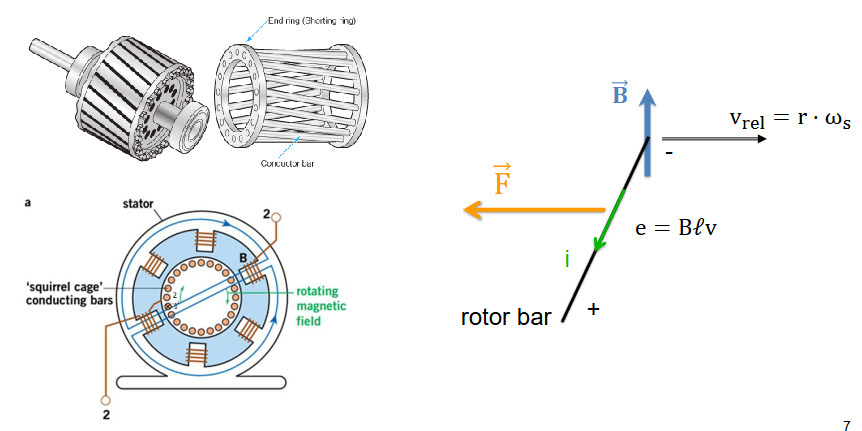
\includegraphics[width=0.6\textwidth]{assets/inductiemachinerotor.png}
  \caption{Rotor inductiemachine}
  \label{fig:inductiemachinerotor.png}
 \end{figure}

De wetten die dit dus allemaal mogelijk maakten zijn:

\begin{itemize}
 \item Wet van Faraday Lenz: $e = B \cdot l \cdot v$
 \item Wet van Lorentz: $F = B \cdot l \cdot I$
 \item Wet van Ohm: $i = \frac{e}{R}$
 \item Wet van Newton:
 $\sum T = J \cdot \alpha$ ($J$ = traagheidsmoment, $\alpha$ = hoekversnelling)
\end{itemize}

\subsection{Slip}
Bij de inductiemachine komt de term 'slip' ook vaak aan bod, dit is omdat de spanning
enkel geïnduceerd wordt als er een snelheidsverschil is tussen het veld en de rotor en de
slip wordt letterlijk geclassificeerd als \textit{het snelheidsverschil tussen het
draaiveld en de rotor.} Daarom kan de slip wiskundig als volgt ook beschreven worden:
\begin{align*}
 s = \frac{n_s - n}{n_s} \cdot 100\% = \frac{\omega_s - \omega}{\omega_s} \cdot 100\%
\end{align*}
Typisch is de slip rond de 3\%, 10\% wordt al als veel beschouwd.
Het is eigelijk een andere uitdrukking voor snelheid, daarom kan het ook geplot worden met
het koppel in een koppel-slip karakteristiek zoals in volgende figuur:

\begin{figure}[H]
  \centering
  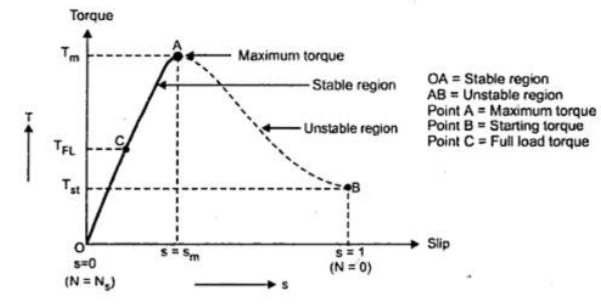
\includegraphics[width=0.6\textwidth]{assets/koppelslip.png}
  \caption{Koppel-slip karakteristiek van een inductiemachine}
  \label{fig:koppelslip.png}
 \end{figure}

We zien hier dat we bij een slip van 0 geen koppel hebben, dit is logisch want op dat
moment draaien we aan synchrone snelheid waardoor dus geen geïnduceerde spanning is.
Bij een slip van 1 hebben we eigelijk gewoon een stilstaande rotor, het draaiveld van de
stator draait hier wel nog.
Voor kleine slippen zoals we zien is er eigelijk een lineair verband met het koppel.

\subsection{Rotorveld}
Aangezien er een stroom in de rotor is zorgt deze ook voor een magnetisch veld via de wet
van Ampère.
Dit veld een een beetje effect op het resulterend draaiveld, maar hoe groter deze stroom
hoe groter dat effect, dit is dus eigelijk zoals ankerreactie.
Door de slip is er een verschil in snelheid, we zeggen hier dat het draaiveld aan 1500
tr/min draait en de rotor aan 1480 tr/min.

\subsubsection{Buitenstaande waarnemen (stator)}
Als je als buitenstaande waarnemer gaat kijken naar de inductie machine dan ziet die
gewoon alle stromen van in de volgende figuur draaien aan een snelheid van 1500 tr/min,
terwijl de rotorstroom $I_R$ zich in de rotor bevind, dit is omdat het geïnduceerd wordt
door dat draaiveld dat het dan eigelijk iets sneller draait als de rotor zelf.

\begin{figure}[H]
  \centering
  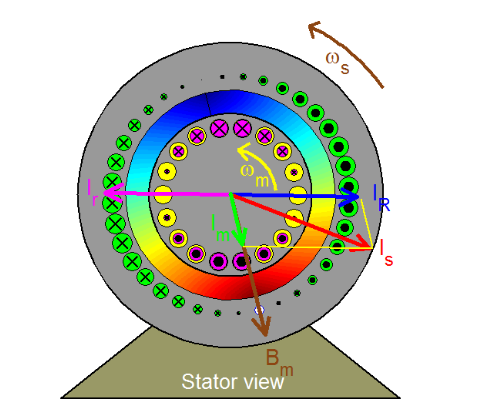
\includegraphics[width=0.4\textwidth]{assets/statorviewinductiemachine.png}
  \caption{Stator view van een inductiemachine, buitenstaander waarnemer}
  \label{fig:statorviewinductiemachine.png}
 \end{figure}

\subsubsection{Synchronous view (jij rijdt mee op het draaiveld)}
Als we nu als waarnemer OP de machine gaan, eigelijk mee met het draaiveld, dan is
$\omega = 0$, het draaiveld is stil vanuit ons standpunt, maar sinds de rotor dat tempo
niet haalt gaat het eigelijk traag lijken weg te glijden, waardoor de stroom in de
rotorstaven traag varieert.
Dit is dus gelinkt aan die slip, die stroom is een geïnduceerde AC stroom dat niet aan
50Hz is maar trager dan het draaiveld.

\begin{figure}[H]
  \centering
  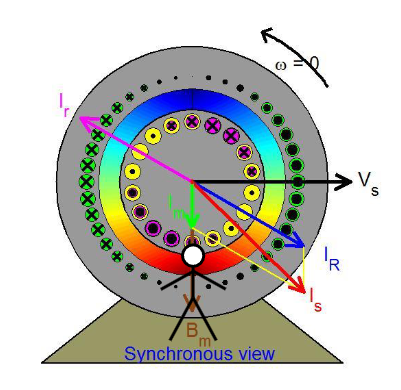
\includegraphics[width=0.4\textwidth]{assets/synchronoyusviewinductiemachine.png}
  \caption{Synchronous view van een inductiemachine, waarnemer die mee rijdt op het
  draaiveld}
  \label{fig:synchronoyusviewinductiemachine.png}
 \end{figure}

\subsubsection{Rotor view (jij rijdt mee op de rotor)}
Als we nu als waarnemer op de rotor gaan, lijkt het draaiveld aan 20 tr/min te passeren,
dus aan $\omega_{sl} = 20 tr/min$, dit is die slip.
Als we dit omzetten naar frequentie geeft dit exact volgende relatie:
\begin{align*}
    f_r = s \cdot f_s
\end{align*}
De rotor frequentie is een lage frequentie, dus niet 50Hz, dit is een belangrijke formule
om te onthouden.

\begin{figure}[H]
  \centering
  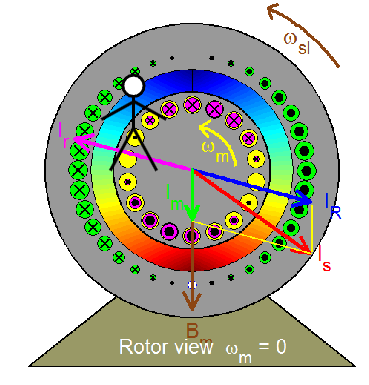
\includegraphics[width=0.4\textwidth]{assets/rotorviewinductiemachine.png}
  \caption{Rotor view van een inductiemachine, waarnemer die mee rijdt op de rotor}
  \label{fig:rotorviewinductiemachine.png}
 \end{figure}

\subsection{Kenplaat oefening}
Dit thema is een beetje messy als het neer komt op de oefeningen, ze zijn niet zomaar
allemaal vanachter op het eind van dit thema, ik ga de meeste hiervan dus tussen de
theorie plaatsen in de zelfde volgorde als hoe ze in de les aan bod kwamen.
Ik raad aan om ze ook zo te maken in plaats van te wachten tegen dat je het hoofdstuk van
inductiemachines af hebt want dit is veel.

\begin{oefenblok}[Oefening Kenplaat Inductiemachine]
\textbf{Opgave:}
\begin{figure}[H]
  \centering
  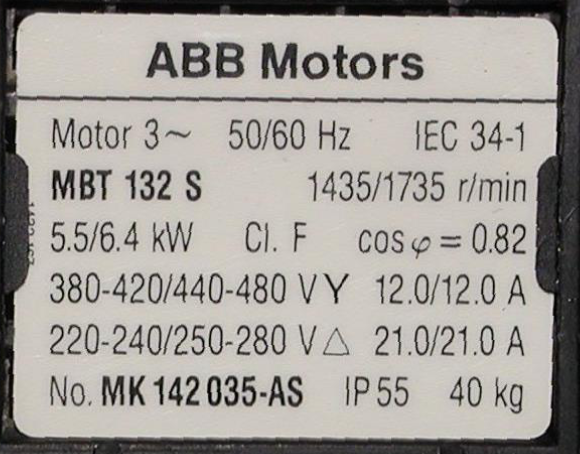
\includegraphics[width=0.5\textwidth]{assets/kenplaatoefeninginductiemachine.png}
  \caption{Kenplaat oefening inductiemachine}
  \label{fig:kenplaatoefeninginductiemachine.png}
 \end{figure}
\begin{itemize}
 \item a) Determine: p, $n_s$, $s_{nom}$, $\eta_{nom}$, $T_{nom}$
 \item b) The load torque is half of the nominal torque. Determine the output power.
 \item c) The rotor is driven (i.e.
 generator) with a torque of 25Nm.
 Determine the rotor speed.
\end{itemize}
\textbf{Oplossing:}
\newline
\textbf{a)}
\newline
Er is geen ronde synchrone snelheid gegeven, er is wel gegeven dat het nominale toerental
$n_{nom} = 1435 tr/min$ is.
Dit kan alleen overkomen met een 4 polige machine want deze heeft een synchrone snelheid
van 1500 tr/min.
Dit toerental van 1435 komt overeen met een frequentie van 50Hz, dus die 1500 kunnen we
ook dubbel checken met:
\begin{align*}
    n_s = \frac{60 \cdot f}{p} = \frac{60 \cdot 50 Hz}{4} = 750 tr/s = 1500 tr/min
\end{align*}
De nominale slip vinden we dan met de eerder geziene formule:
\begin{align*}
    s_{nom} = \frac{n_s - n_{nom}}{n_s} = \frac{1500 - 1435}{1500} = 0.0433 = 4.33\%
\end{align*}
Het nominaal rendement vinden we met de formule:
\begin{align*}
    \eta_{nom} = \frac{P_{out}}{P_{in}} = \frac{P_{mech}}{P_{el}}
\end{align*}
Het mechanisch vermogen kan afgelezen worden van de kenplaat en bedraagt 5.5 kW.
Het elektrisch vermogen kunnen we berekenen met de formule:
\begin{align*}
    P_{el} = \sqrt{3} \cdot V_L \cdot I_L \cdot \cos(\varphi)
\end{align*}
$V_L$ en $I_L$ kunnen we aflezen, we gaan dit doen voor Ster.
Aangezien de lijnspanning een range heeft pakken we het gemiddelde hiervan (400V) en de
lijnstroom bij ster bedraagt 12A.
De arbeidsfactor kunnen we ook aflezen (0.82).
Invullen geeft:
\begin{align*}
    P_{el} = \sqrt{3} \cdot 400 V \cdot 12 A \cdot 0.82 = 6.82 kW
\end{align*}
Het nominaal rendement is dus:
\begin{align*}
    \eta_{nom} = \frac{5.5 kW}{6.82 kW} = 0.806 = 80.6\%
\end{align*}
Het nominaal koppel kunnen we berekenen met de formule:
\begin{align*}
    T_{nom} = \frac{P_{mech}}{\omega_{nom}} = \frac{5.5 kW}{2 \cdot \pi \cdot \frac{1435 tr/min}{60}} = 36.7 Nm
\end{align*}
\textbf{b)}
\newline
Als we het koppel van de last gaan halveren, gaat bij benadering het vermogen ook
halveren, maar het is dus eigelijk fout om het zo te doen want $\omega$ vernaderd ook en
er zal dus minder slop nodig zijn omdat gehalveerd koppel te leveren.
Dit gaan we nu ook proberen na gaan.

Wat we gaan doen is kijken naar de T-n grafiek, want in de buurt van $n_s$ is deze kromme
eigelijk een rechte lijn (zoals bij de T-s grafiek).
2 punten van deze rechte kennen we, namelijk het punt (n = 1435; T = 36,7) en (n = 1500; T
= 0).
Via interpolatie vinden we zo welk toerental bij het gehalveerd koppel hoort.
Hiermee vinden we juiste $\omega$ en zo het juiste vermogen bij een gehalveerd koppel:
\begin{figure}[H]
  \centering
  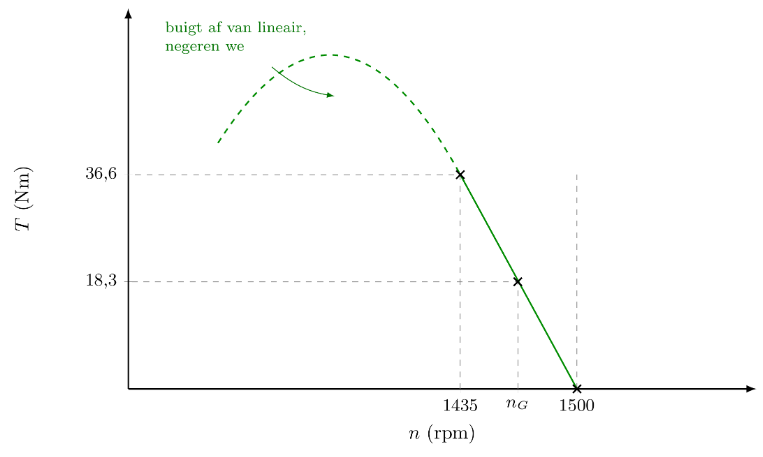
\includegraphics[width=0.6\textwidth]{assets/AIgeneratedgrafieklineairgebiedTn.png}
  \caption{Lineair verloop van T-n karakteristiek in het gebied van nominale snelheid (AI
  gegenereerd maar is juist)}
  \label{fig:AIgeneratedgrafieklineairgebiedTn.png}
 \end{figure}
\begin{align*}
 n_G = n_1 + \frac{T_G - T_1}{T_2 - T_1} \cdot (n_2 - n_1) = 1435 + \frac{18.35 - 36.7}{0 - 36.7} \cdot (1500 - 1435) = 1467 tr/min
\end{align*}
Hiermee kunnen we het mechanisch vermogen berekenen:
\begin{align*}
    P_{mech} = T_G \cdot \omega_G = 18.35 Nm \cdot 2 \cdot \pi \cdot \frac{1467 tr/min}{60} = 2.82 kW
\end{align*}
Dit is inderdaad ongeveer de helft van het nominaal vermogen, maar niet exact want de
snelheid is ook veranderd.
\newline
\textbf{c)}
Nu wordt de rotor aangedreven met een koppel van 25Nm, dit is dus generatorwerking.
Dit is een negatief koppel op de grafiek maar gaat de snelheid trager of sneller zijn dan
de synchrone snelheid?
Wel, een aangedreven rotor die generator wordt, kan alleen als hij sneller draait dan het
draaiveld dus het is groter, we kunnen de lineaire relatie dan onder de n-as doortrekken
en de snelheid berekenen bij -25Nm:
\begin{align*}
    n_C = n_1 + \frac{T_C - T_1}{T_2 - T_1} \cdot (n_2 - n_1) = 1435 + \frac{-25 - 36.7}{0 - 36.7} \cdot (1500 - 1435) = 1544 tr/min
\end{align*}
\begin{figure}[H]
  \centering
  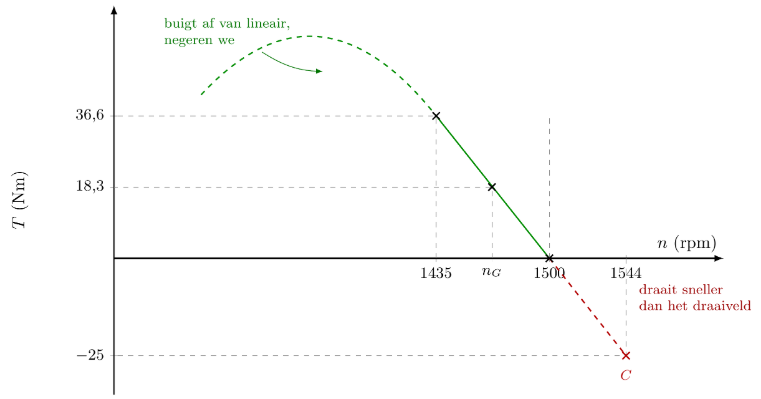
\includegraphics[width=0.6\textwidth]{assets/AIgeneratedgrafieklineairgebiedgenerator.png}
  \caption{Lineair verloop van T-n karakteristiek in het gebied van generatorwerking (AI
  gegenereerd maar is juist)}
  \label{fig:AIgeneratedgrafieklineairgebiedgenerator.png}
 \end{figure}
\end{oefenblok}

\subsection{Nominaal werkingspunt}
In volgende figuren zien we verschillende karakteristieken met hun aangeduidde nominale
werkingspunten:

\begin{figure}[H]
  \centering
  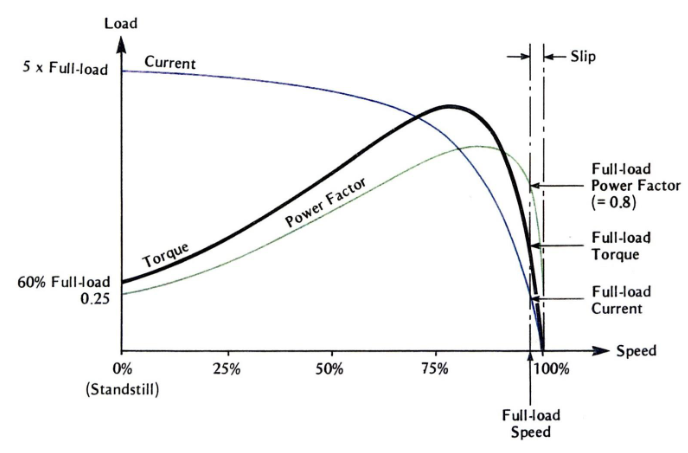
\includegraphics[width=0.6\textwidth]{assets/nominalewerkingspuntkarakteristieken.png}
  \caption{Stroom, koppel en arbeidsfactor karakteristiek}
  \label{fig:nominalewerkingspuntkarakteristieken.png}
 \end{figure}

We zien dat bij vollast de arbeidsfactor goed is als die rond de 0.8 ligt.
Aan de grafiek zien we ook het grootste nadeel van de inductie motor; namelijk de hoge
startstroom.

\section{Equivalent schema}
Voor het opstellen van het equivalent schema van de inductiemachine gaan we niet van 0
beginnen, we gaan een analogie zoeken en hiernaar toe aanpassen.
We gebruiken hier die van de transformator want eigelijk is de inductiemachine een soort
van transfo want we hebben hier ook eigelijk een spanning dat wordt geïnduceerd van de ene
kant naar de andere kant.
Hier is dit dan met een stator en een rotor i.p.v.
een primaire en secundaire wikkeling.
We gaan hierbij van uit van een symmetrisch net, en ook van een sinusoïdaal magnetisch
veld in de luchtspleet.
Het schema dat we opstellen is hier ook een éénfasig equivalent, let hier mee dus op want
een inductie motor is 3-fasig.
Tussen de transfo en de inductie machine zijn echter 3 grote verschillen:

\begin{itemize}
    \item De rotor is kortgesloten, dus er is geen spanning dat we kunnen meten aan de
    rotor, dit is dus een verschil met de transfo.
    Hierdoor kan er wel een stroom $I_r$ lopen zonder dat er iets extern aangesloten moet
    worden, het loopt door de geînduceerde $E_R$ door de impedantie van de rotor
    \item Er werkt een andere frequentie in de rotor dat verschilt van de stator
    \item De spoel $L_m$ (magnetiseringstroom) is veel kleiner hier, waardoor we veel meer
    nullaststroom krijgen.
    (Bij een motor is dit niet zo een groot probleem, bij een transfo wel)
\end{itemize}

\begin{figure}[H]
  \centering
  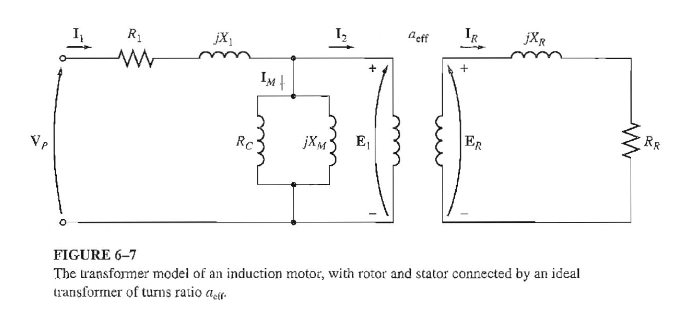
\includegraphics[width=0.8\textwidth]{assets/transfoanalogieinductiemachine.png}
  \caption{Transfo analogie inductiemachine}
  \label{fig:transfoanalogieinductiemachine.png}
 \end{figure}

Het equivalent schema van de inductiemachine is dus als volgt:

\begin{figure}[H]
  \centering
  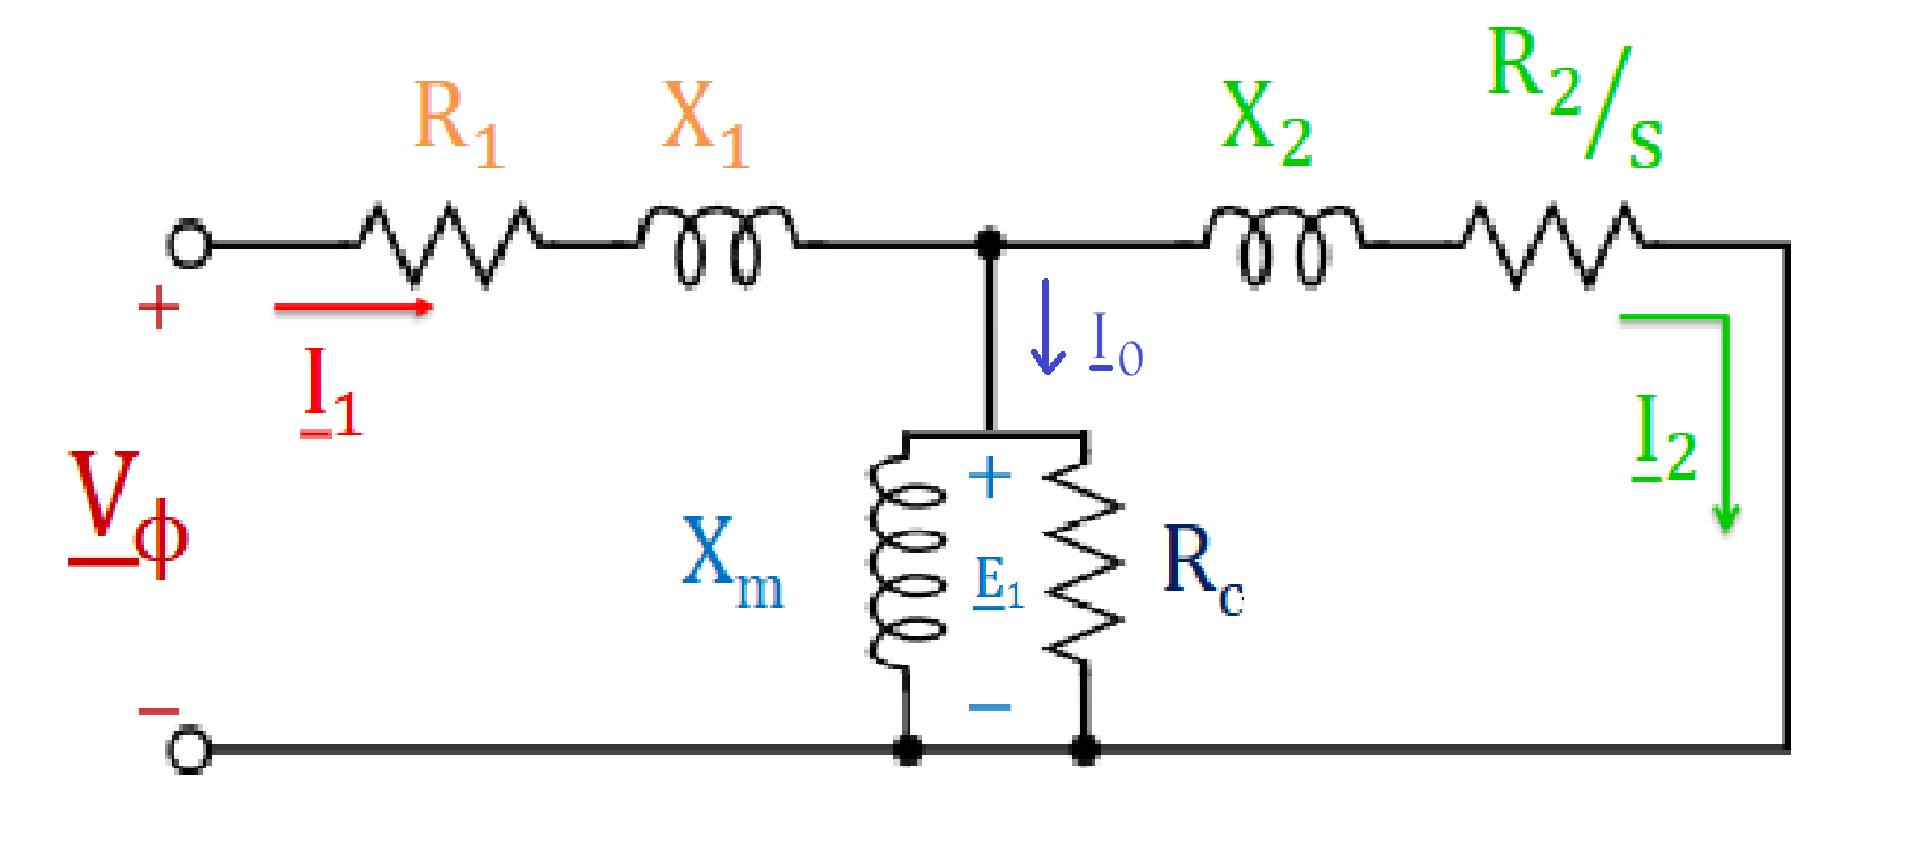
\includegraphics[width=0.8\textwidth]{assets/equivalentschemainductiemotor.png}
  \caption{Equivalent schema inductiemachine}
  \label{fig:equivalentschemainductiemotor.png}
 \end{figure}

Hierbij is:

\begin{itemize}
 \item \textbf{$R_1$} de fysieke weerstand van de statorwikkeling (koperverlies)
 \item \textbf{$X_1$} de lekreactantie van de stator, dit gaat door de stator en bereikt
 (niet volledig) de rotor
 \item \textbf{$R_C$} het model van de ijzerverliezen (kern), dit is geen echte weerstand,
 gewoon een model om deze verliezen elektrisch voor te stellen!
 (Wervel en hysteresis eigelijk)
 \item \textbf{$X_m$} de mutuele/magnetiserende reactantie
 \item \textbf{$E_1$} de interne spanning over de parallele tak van $R_C$ en $X_m$
 \item \textbf{$X_2$} de lekreactantie van de rotor, dit gaat door de rotor en bereikt
 (niet volledig) de stator
 \item \textbf{$R_2$} de fysieke weerstand van de rotorwikkeling (koperverlies) (Er staat
 wel $\frac{R_2}{s}$ in het schema, hier kom ik zometeen op terug)
 \item \textbf{$I_1$} de stroom door de statorwikkeling
 \item \textbf{$I_2$} de stroom door de rotorwikkeling
 \item \textbf{$I_0$} de nullaststroom, dit is de stroom die loopt door $R_C$ en $X_m$,
 deze kan tot 30\% van de nominale stroom zijn, want de luchtspleet zorgt dat we veel
 stroom nodig hebben
\end{itemize}

Liefst hebben we $X_1$ en $X_2$ zo klein mogelijk en $X_m$ zo groot mogelijk (logisch,
minder verlies en minder stroom), bij de transfo gelde ook dat R1 en R2 gelijkmatig
verdeeld werden maar dit is nu niet meer zo aangezien da stator en de rotor uit
verschillend materiaal bestaan.

\subsection{Waarom staat er $\frac{R_2}{s}$ i.p.v. $R_2$?}
Dit is het lastigste stuk van het schema, dus we bouwen het stap voor stap op.

Het probleem:
de rotor werkt niet aan de statorfrequentie $f_s$, maar aan de rotorfrequentie
$f_r = s \cdot f_s$ (bv.
50Hz bij stilstand, maar slechts 1 à 2Hz bij normaal bedrijf met een kleine slip).
We willen echter maar 1 schema tekenen, op 1 frequentie (die van de stator).
Daarom moeten we de rotorvergelijking eerst herschrijven.

Aan de eigen (rotor)frequentie geldt gewoon de wet van Ohm over de kortgesloten rotorlus:
\begin{align*}
    E_R = R_R \cdot I_R + jX_R \cdot I_R
\end{align*}
Hierbij is $X_R = s \cdot X_{R0}$, met $X_{R0}$ de rotorreactantie bij stilstand (dus bij
50Hz, $s=1$).
Ook $E_R$ zelf is rechtevenredig met de slip:
$E_R = s \cdot E_{R0}$ (logisch, want $e = B\ell v$:
hoe groter de relatieve snelheid tussen rotor en draaiveld, hoe groter de geïnduceerde
spanning).

Vullen we dit in en delen we alles door $s$, dan krijgen we:
\begin{align*}
    s \cdot E_{R0} = R_R \cdot I_R + j s X_{R0} \cdot I_R \quad\Rightarrow\quad E_{R0} = \left(\frac{R_R}{s} + jX_{R0}\right) \cdot I_R
\end{align*}
En daar komt die $\frac{R_2}{s}$ dus vandaan:
het is geen aparte fysische grootheid, het is gewoon het resultaat van die deling door
$s$, nodig om het frequentieverschil tussen rotor en stator weg te werken zodat we alles
op de statorfrequentie kunnen tekenen.
$\frac{R_2}{s}$ in het equivalent schema schrijven compenseert dus voor die verschillde
frequenties.
Het is dus eigelijk gelijk aan:
\begin{align*}
   \frac{R_2}{s} = R_2 + (\frac{1-s}{s}) \cdot R_2 = \underbrace{R_2 + {R'}_{load}}_{\text{in serie}}
\end{align*}
Die $R'_{load}$ is dus de weerstand die de rotor moet overwinnen om het koppel te leveren,
en die is groter naarmate de slip kleiner wordt (want dan draait de rotor sneller, dus
moet hij meer kracht leveren).
Bij stilstand ($s=1$) is er geen extra weerstand, bij synchrone snelheid ($s=0$) is de
weerstand oneindig groot (want dan kan er geen stroom meer lopen in de rotor).

\begin{warningbox}[Hier zijn het fasegrootheden, geen lijn grootheden!]
    Alle grootheden weergegeven in het equivalent schema zijn fase grootheden, niet lijn
    grootheden.
    Bij kenplaten wordt wel alles in lijn grootheden weergegeven, dus let hier goed op bij
    het oplossen van oefeningen.
\end{warningbox}

\section{Vermogensbalans}
Nu gaan we kijken naar het vermogen balans, en dus ook waar precies in de inductiemachine
alle verliezen bevinden.
We bespreken ook de formules, we gaan dit allemaal doen aan de hand van een soort van
Sankey-diagram zoals te zien in de volgende figuur:

\begin{figure}[H]
\centering
\begin{tikzpicture}[
    node distance=0.25cm,
    block/.style={single arrow, draw=black, thick, minimum height=1.5cm,
                  minimum width=1.7cm, single arrow head extend=0.25cm,
                  font=\bfseries, align=center, inner sep=2pt},
    stage/.style={circle, draw=black, thick, fill=violet!60,
                  minimum size=1.6cm, font=\bfseries\footnotesize, align=center},
    formula/.style={align=center, font=\small},
    lossarrow/.style={single arrow, draw=black, thick, fill=red!35,
                       minimum height=0.9cm, minimum width=0.35cm,
                       single arrow head extend=0.12cm, rotate=-90},
]

\node[block, fill=orange!55] (Pin) {$P_{in}$};
\node[stage, right=of Pin] (stator) {Stator};
\node[block, fill=blue!30, right=of stator] (Ps) {$P_{S}$};
\node[stage, right=of Ps] (rotor) {Rotor};
\node[block, fill=green!40, right=of rotor] (Pconv) {$P_{conv}$};
\node[stage, right=of Pconv] (shaft) {Shaft};
\node[block, fill=green!40, right=of shaft] (Pout) {$P_{mech}$};

\node[formula, above=0.35cm of Pin] {$\sqrt{3}V_TI_T\cos\varphi = 3V_\phi I_1\cos\varphi$\\$\Vert$};
\node[formula, above=0.35cm of Ps] {$3\dfrac{R_2}{s}I_2^2$\\$\Vert$};
\node[formula, above=0.35cm of Pconv] {$T_{ind}\cdot\omega$\\$\Vert$\\$3R_2\left(\dfrac{1-s}{s}\right)I_2^2$};
\node[formula, above=0.35cm of Pout] {$T_{load}\cdot\omega$\\$\Vert$};

\node[lossarrow] (lcus) at ($(stator.south)+(-0.6,-0.7)$) {};
\node[formula, below=0.45cm of lcus] {$P_{Cu,s}$\\$\Vert$\\$3I_1^2R_1$};

\node[lossarrow] (lfe) at ($(stator.south)+(0.6,-0.7)$) {};
\node[formula, below=0.45cm of lfe] {$P_{Fe}$\\$\Vert$\\$3\dfrac{E_1^2}{R_C}$};

\node[lossarrow] (lwr) at ($(rotor.south)+(0,-0.7)$) {};
\node[formula, below=0.45cm of lwr] {$P_{Cu,r}$\\$\Vert$\\$3I_2^2R_2 = s \cdot P_S$};

\node[lossarrow] (lfw) at ($(shaft.south)+(0,-0.7)$) {};
\node[formula, below=0.45cm of lfw] {$P_{wr} + P_w + P_{str}$};

\end{tikzpicture}
\caption{Vermogensbalans van de inductiemachine}
\label{fig:vermogensbalans}
\end{figure}

Wat we hier zien is dat we starten bij het elektrisch vermogen $P_{el}$ dat in de stator
wordt geleverd, dit is het vermogen dat we dus van het net halen.
In de stator zijn er wel een paar verliezen, namelijk de ijzerverliezen $P_{Fe}$ en de
koperverliezen $P_{Cu,s}$.
Het vermogen dat overblijft wordt overgedragen naar de rotor, dit overgedragen vermogen
heet het luchtspleetvermogen $P_S$.
In de rotor zijn er ook weer koperverliezen $P_{Cu,r}$.
Het theoretisch mechanisch vermogen dat kan overgedragen worden naar de as is het
conventioneel vermogen $P_{conv}$.
Om van de as naar het effectief mechanisch vermogen $P_{mech}$ te gaan zijn dus echter een
paar verliezen nog.
We hebben wrijvingsverliezen $P_{wr}$, deze zijn vooral warmte, dit is vooral in de lagers
maar komt in totaal weinig voor in de inductiemachine, dan hebben we ook windingsverliezen
$P_w$, dit zijn aerodynamische wrijvingsverliezen door lucht en uiteindelijk nog
strooiverliezen $P_{str}$, dit zijn alle andere verliezen zoals bvb.
harmonischen ofzo, deze zijn in totaal echter heel klein (1\% ofzo).

In de stator zijn er trouwens meer ijzerverliezen want de frequentie in de rotor is lager
en die ijzerverliezen zijn frequentie afhankelijk, want de frequentie bepaald hoeveel het
magnetisch veld op en neer gaat (hysteresis).

\subsection{Soorten metingen}
Net zoals bij de synchrone machine willen we de parameters van het equivalent schema
kunnen bepalen, hiervoor zijn er een paar metingen nodig indien deze niet allemaal gekend
zijn.

\subsubsection{DC weerstandsmeting}
Hier gaan we de weerstandsmeting voor $R_1$ doen, dit doen we terwijl de motor in
stilstand is.
Dus $s = 1$.
We hangen dan een DC bron aan 2 fases van de stator zoals in volgende figuur:

\begin{figure}[H]
  \centering
  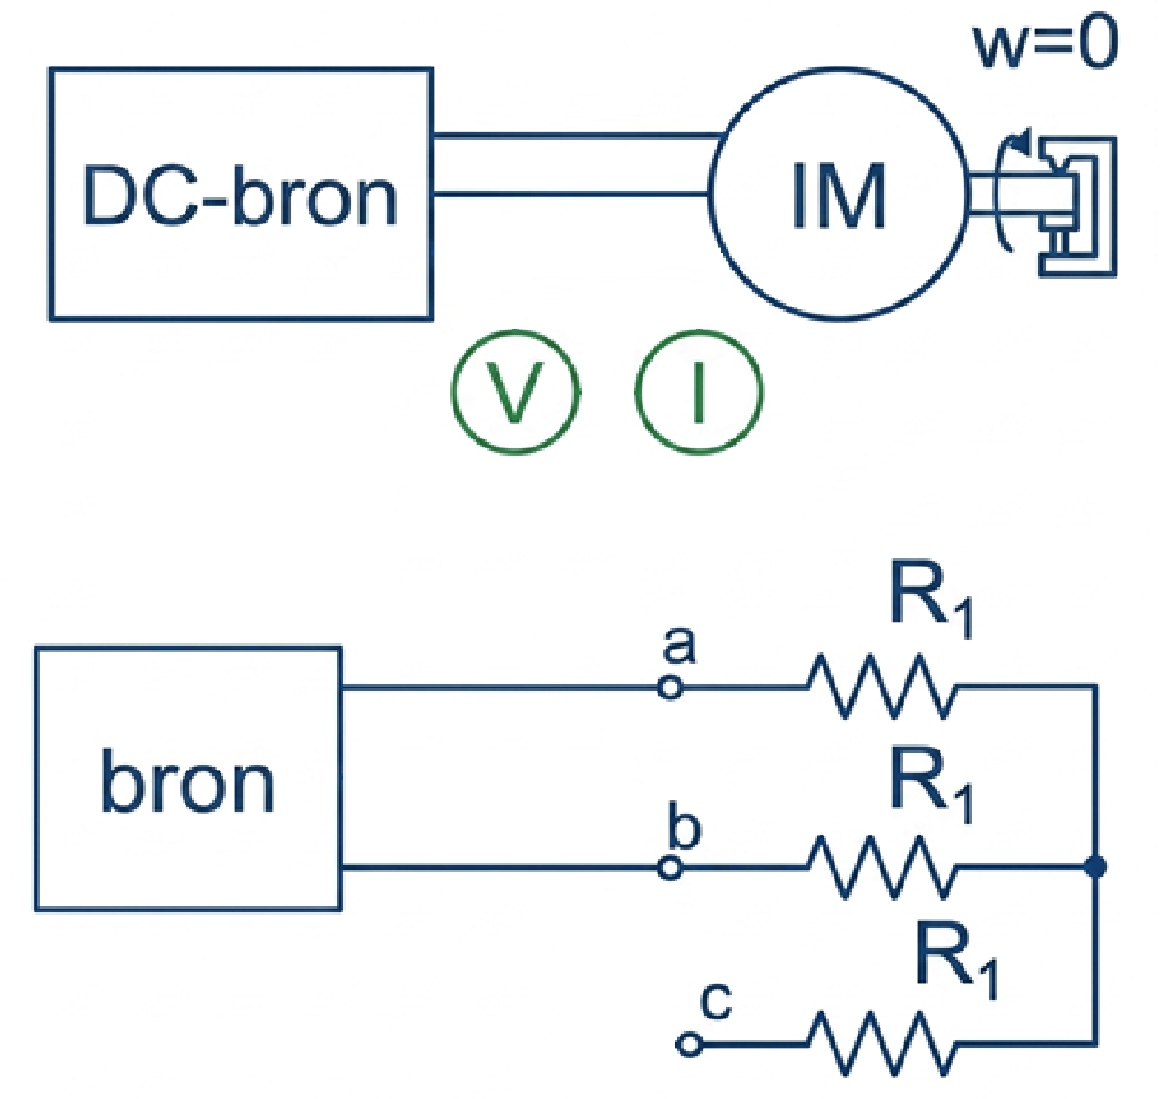
\includegraphics[width=0.4\textwidth]{assets/opstellingdcweerstandsmeting.png}
  \caption{Opstelling DC weerstandsmeting}
  \label{fig:opstellingdcweerstandsmeting.png}
 \end{figure}

We gaan hierdan dus een DC stroom door 2 $R_1$ weerstanden sturen, doordat het DC is gaan
de spoelen geen effect hebben en kunnen we gewoon de weerstand meten zoals we zien in
onderstaande schema:

\begin{figure}[H]
  \centering
  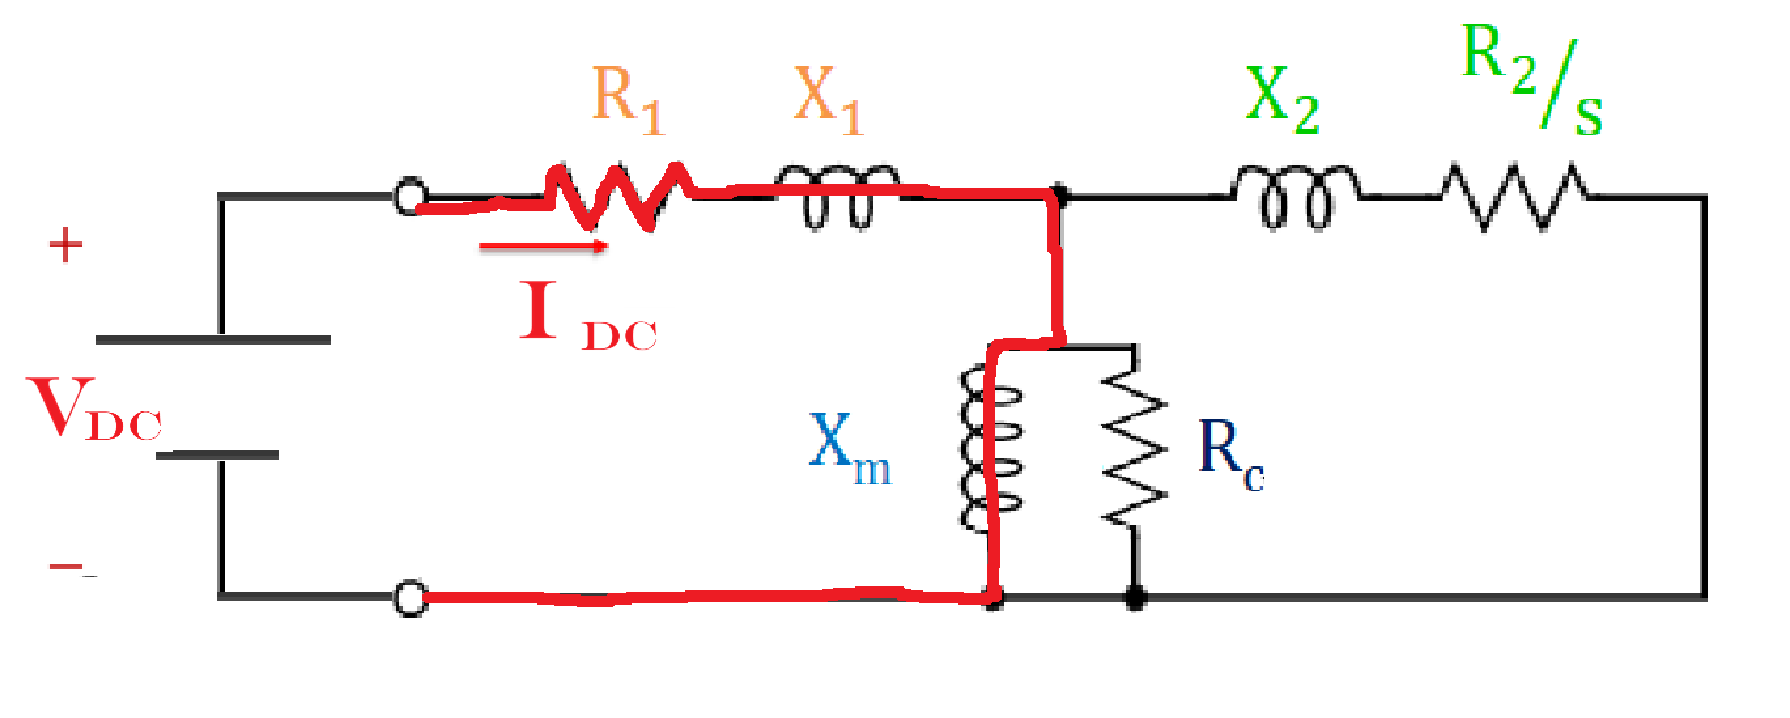
\includegraphics[width=0.8\textwidth]{assets/stroomverloopdcweerstandsmetong.png}
  \caption{DC stroom weerstandsmeting}
  \label{fig:stroomverloopdcweerstandsmetong.png}
 \end{figure}

Let dus wel op want hierboven is het een 1-fasig schema, ook is de onderste klem van de
figuur hierboven eigelijk de neuter, in de 1ste figuur zagen we dat we door 2 $R_1$
weerstanden gingen dus de $R_1$ weerstand kan berekend worden met:
\begin{align*}
    R_1 = \frac{V_{DC}}{2 \cdot I_{DC}}
\end{align*}
Dit is een goede benadering van de weerstand, in het echt verschilt deze nog een beetje
want bij AC heb je ook nog skin-effect.
Zie ook dat je deze proef als laatste doet want eigelijk wil je deze weerstand meten op de
steady-state temperatuur van de machine want normaal als hij draait warmt hij op en dan is
de weerstand anders.

\subsubsection{Nullastproef}
Bij de nullastproef is het doel om de verliezen te meten (de wrijvings en ijzerverliezen).
Hier laten we de motor op volle snelheid draaien ($n_s$) en we hangen er geen last aan ook
dus $T = 0$, ook veronderstellen we geen mechanische verliezen, dit betekent dat
$R'_{load}$ naar oneindig gaat (open keten).
De nominale spanning sluiten we aan en we gaan dan de spanning, stroom en vermogen meten
zoals we zien in de volgende opstelling:

\begin{figure}[H]
  \centering
  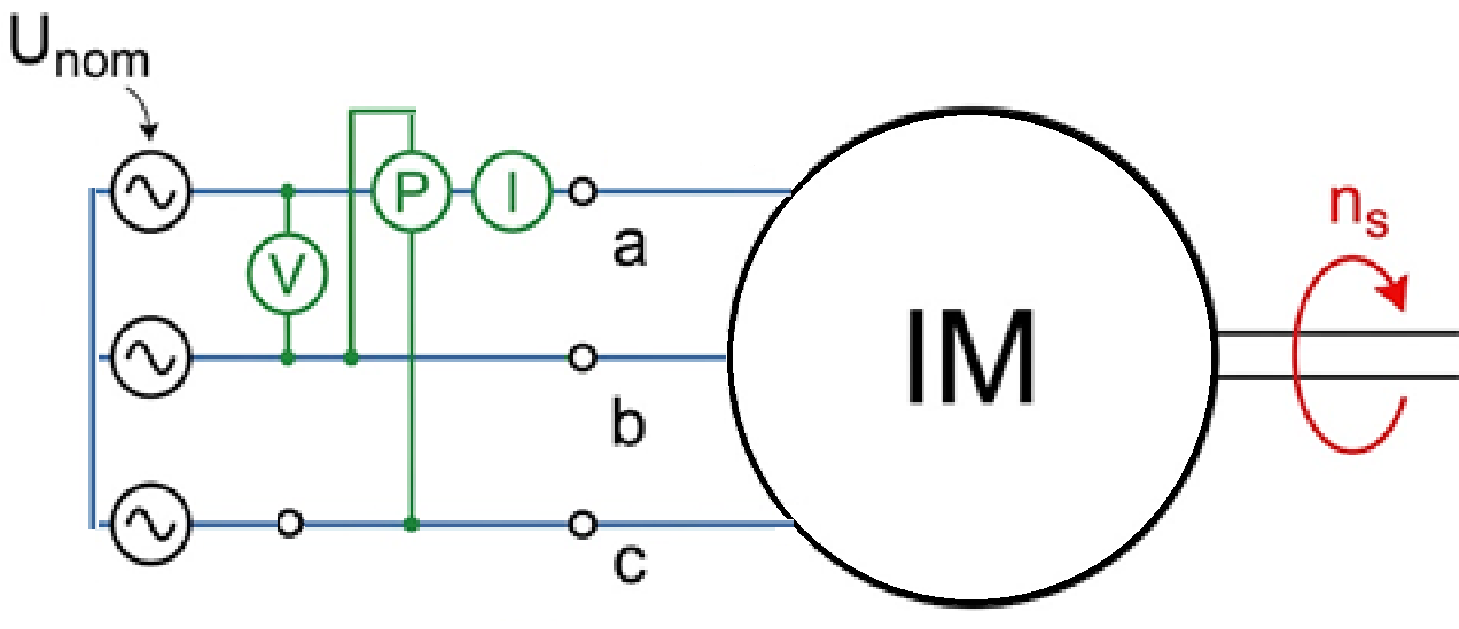
\includegraphics[width=0.6\textwidth]{assets/opstellingnullastproef.png}
  \caption{Opstelling nullastproef inductiemachine}
  \label{fig:opstellingnullastproef.png}
 \end{figure}

Doordat het op synchrone snelheid is gaat er dus ook geen spanning geïnduceerd worden en
geen stroom vloeien (ook logisch als die weerstand oneindig is) dus het hele rotor
gedeelte van het equivalent schema valt dus weg, oftewel zoals ik net eigelijk al zei, dit
wordt een open keten.
Het equivalent schema voor deze proef ziet er dan zo uit:

\begin{figure}[H]
  \centering
  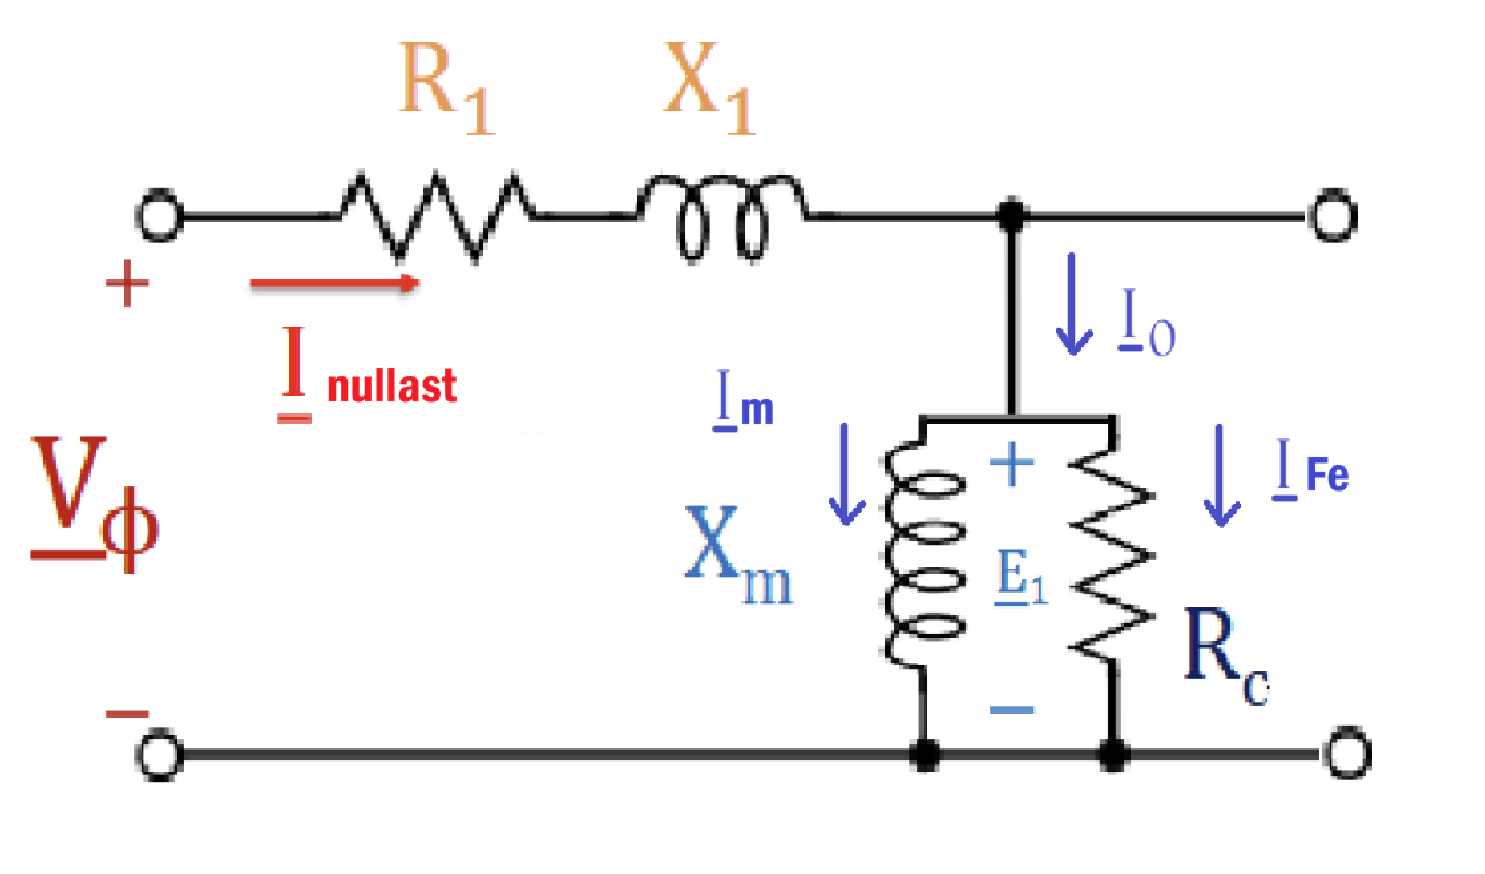
\includegraphics[width=0.6\textwidth]{assets/equivschemanullastproefIM.png}
  \caption{Equivalent schema nullastproef inductiemachine}
  \label{fig:equivschemanullastproefIM.png}
 \end{figure}

($I_{Nullast}$ is eigelijk exact hetzelfde als $I_0$ in dit equivalent schema)

Als we nu het vermogen meten als $P_{Nullast}$ dan is dit de som van de ijzerverliezen en
de wrijvingsverliezen:
\begin{align*}
    P_{Nullast} = P_{R_1} + P_{R_{Fe}} = \underbrace{3 \cdot I_{Nullast}^2 \cdot R_1}_{\text{Kunnen we berekenen}} + 3 \cdot \frac{E_1^2}{R_{Fe}}
\end{align*}
Aangezien de spanningsval over $R_1$ en $X_1$ klein is tegenover $V_\phi$ kunnen we
eigelijk de benadering maken dat $E_1 \approx V_\phi$ en dus kunnen we $R_{Fe}$ berekenen
met:
\begin{align*}
    R_{Fe} = \frac{3 \cdot V_\phi^2}{P_{Nullast} - 3 \cdot I_{Nullast}^2 \cdot R_1}
\end{align*}
Met deze zelfde aanname ($R_{Fe}, X_m >> R_1, X_1$ en $E_1 \approx V_\phi$) kunnen we ook
$X_1 + X_m$ berekenen met:
\begin{align*}
    X_1 + X_m = \frac{3 \cdot V_\phi^2}{Q_{Nullast}} = \frac{3 \cdot V_\phi^2}{\sqrt{S_{Nullast}^2 - P_{Nullast}^2}}
\end{align*}
Want $S_{Nullast} = \sqrt{3} \cdot V_L \cdot I_L = 3 \cdot V_\phi \cdot I_0$ en
$Q_{Nullast} = \sqrt{S_{Nullast}^2 - P_{Nullast}^2}$.

\subsubsection{Blokkeerproef (Locked rotor test)}
Hier is het doel om $R_2$ en $X_1 + X_2$ te bepalen.
We blokkeren hierbij de rotor (mechanisch) zodat $n = 0$ en dus $s = 1$.
Daardoor geldt het volgende:
\begin{align*}
    R'_{load} = \frac{1-s}{s} \cdot R_2 = 0
\end{align*}
Dus die tak valt weg, we hebben gewoon de volgende parameters in serie want we gaan de
parallele tak van $R_C$ en $X_m$ verwaarlozen want er zijn hier veel minder verliezen
doordat we spanning gaan verlagen zodat de stroom niet te groot wordt (spanning van 0
regelen tot de nominale waarde van de stroom bereikt wordt).
Er gaat dus weinig vermogen naar die magnetiseertak.
Dus behouden we het volgende equivalent schema:

\begin{figure}[H]
  \centering
  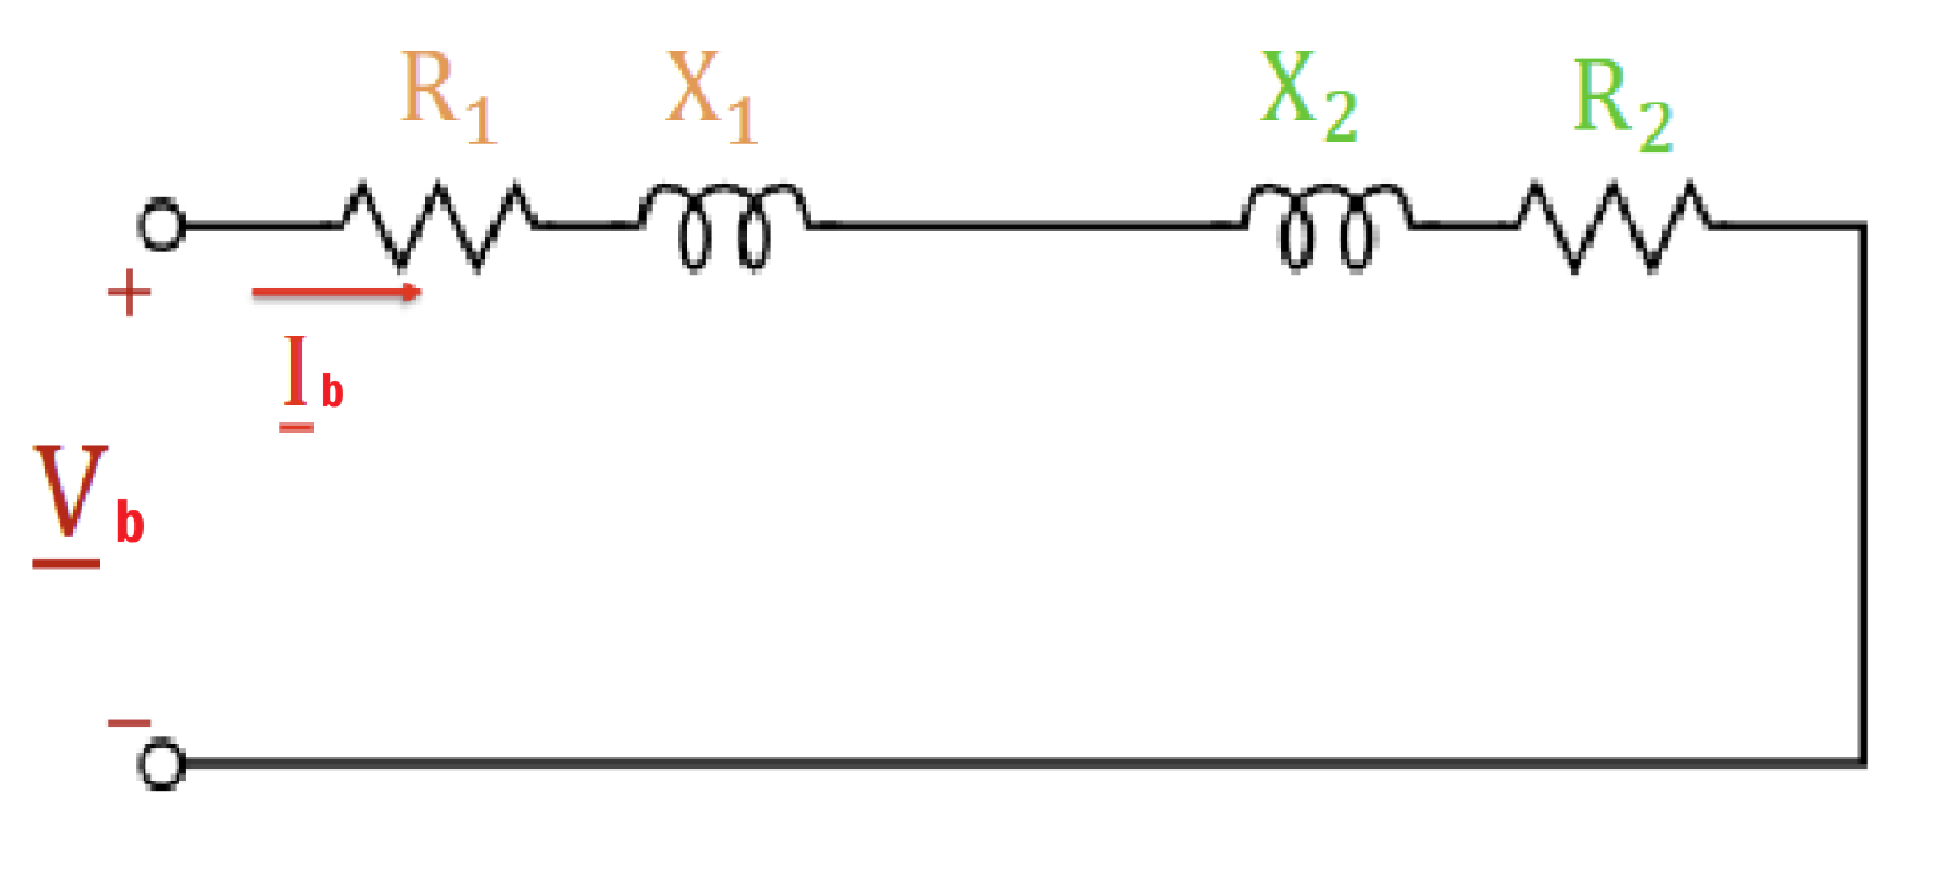
\includegraphics[width=0.6\textwidth]{assets/equivalentschemablokkeerproef.png}
  \caption{Equivalent schema blokkeerproef inductiemachine}
  \label{fig:equivalentschemablokkeerproef.png}
 \end{figure}

Als we nu het vermogen meten als $P_{Blokkeer}$ dan is dit de som van de stator en rotor
verliezen:
\begin{align*}
    P_{Blokkeer} = P_{R_1} + P_{R_2} = \underbrace{3 \cdot I_{Blokkeer}^2 \cdot R_1}_{\text{Kunnen we berekenen}} + 3 \cdot I_{Blokkeer}^2 \cdot R_2
\end{align*}
De stroom weten we ook dus hiermee kunnen we gewoon $R_2$ berekenen.
Je gaat hier zien dat deze inderdaad verschilt van $R_1$ zoals we eerder zeiden.

Met de blokkeer spanning kunnen we totale impedantie berekenen:
\begin{align*}
    Z_{Blokkeer} = \frac{V_{Blokkeer}}{I_{Blokkeer}} = \sqrt{(R_1 + R_2)^2 + (X_1 + X_2)^2}
\end{align*}
Hiermee kunnen we dus $X_1 + X_2$ berekenen.
Oftewel $X_{tot}$, maar we gaan dit $X'_{tot}$ noemen want dit is eigelijk niet de 'echte'
$X_{tot}$.
Deze is namelijk op een frequentie van 15Hz bepaald, niet 60Hz.
Die 15Hz komt van het feit dat normaal de stator 60Hz en de rotor 1Hz ofzo heeft, die 15Hz
dat we nemen is hier een compromis omdat het hier in serie is allemaal.
60Hz zorgt voor teveel skin-effecti in de rotorstaven, 15Hz is een mooie benadering van
het echte lekgedrag.
Omzetten naar het echte kan wel aan de hand van $X = \omega L$ want L is frequentie
onafhankelijk:
\begin{align*}
 X'_{tot} = \omega_{15} \cdot L_{lek, S+R} = 2 \cdot \pi \cdot 15 Hz \cdot L_{lek, S+R} \\
 X_{tot} = X_{lek S+R @60 Hz} = 2 \cdot \pi \cdot 60 Hz \cdot L_{lek, S+R} 
\end{align*}
Dus eigelijk geldt:
\begin{align*}
    X_{tot} = X'_{tot} \cdot \frac{60}{15} = 4 \cdot X'_{tot}
\end{align*}
Om te splitsen naar $X_1$ en $X_2$ gebruiken we standaardverhoudingen genaamd NEMA
verhoudingen, deze bepalen dus de verhouding tussen $X_1$ en $X_2$.
Deze kunnen afgelezen worden uit een tabel, maar als er niks wordt gegeven of gezegd mogen
we een 50/50 verhouding gebruiken:

\begin{figure}[H]
  \centering
  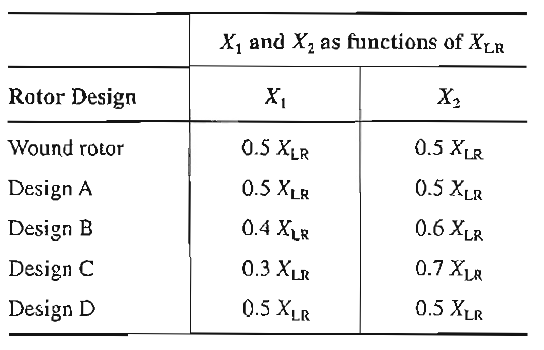
\includegraphics[width=0.4\textwidth]{assets/nemaverhoudingen.png}
  \caption{NEMA verhoudingen voor het splitsen van $X_1$ en $X_2$}
  \label{fig:nemaverhoudingen.png}
 \end{figure}

\section{Koppel-toerentalkarakteristiek}
Dan gaan we nu eens meer uitgebreid kijken naar de koppel-toerentalkarakteristiek van de
inductiemachine.
We hebben al eerder gezien dat deze er ongeveer zo uitziet:

\begin{figure}[H]
  \centering
  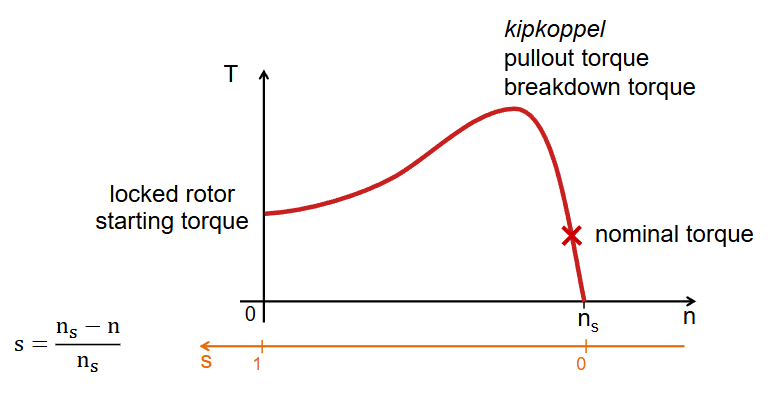
\includegraphics[width=0.6\textwidth]{assets/TNinductiemachine.png}
  \caption{Koppel-toerentalkarakteristiek van de inductiemachine}
  \label{fig:TNinductiemachine.png}
 \end{figure}

Het gebied dat voor die piek van het \textbf{kipkoppel} (maximale koppel dat de machine
kan leveren) is een gebied waar we normaal niet werken.
(Dit zien we later nog waarom niet).
Dit is het \textit{onstabiel gebied}, hier hebben we ons \textbf{startkoppel}.
Van die piek (kipkoppel) tot dat \textit{'nominal torque'} punt (oftewel ons stabiel punt)
hebben we ons \textit{stabiel gebied}, hier kunnen we kortstandig werken want het is
eigelijk overbelasting.
Ideaal werken we rond dat stabiel werkingspunt op het \textbf{nominaal koppel} $T_{nom}$
het gebied hierna willen we niet werken omdat dit een slechte arbeidsfactor heeft.
Deze machine kan zoals we zien rechtstreeks van het net starten.

Om die T-n karakteristiek te berekenen hebben we de formule nodig van het koppel van de
inductiemachine.
We gaan dit doen aan de hand van het conventieel vermogen (we gaan dus van geen verliezen
in de as uit).
We hebben deze formule eerder al gezien eigelijk, nu gaan we tonen vanwaar die komt en hoe
het dus de T-n karakteristiek bepaald.
We weten dus dat dit $P_{conv}$ is:
\begin{align*}
    P_{conv} = T_{ind} \cdot \omega
\end{align*}
In functie van de synchrone snelheid is dit:
\begin{align*}
    P_{conv} = T_{ind} \cdot \omega_s \cdot (1-s)
\end{align*}
Ook weten we dat $P_{conv} = P_S - P_{Cu,r}$ (Zie eerder het vermogen balans) dus:
\begin{align*}
    P_{conv} = P_S - P_{Cu,r} = 3 \cdot I_2^2 \cdot \frac{R_2}{s} - 3 \cdot I_2^2 \cdot R_2 = 3 \cdot I_2^2 \cdot R_2 \left(\frac{1-s}{s}\right)
\end{align*}
Hieruit kunnen we dus het koppel berekenen:
\begin{align*}
    T_{ind} = \frac{P_{conv}}{\omega_s \cdot (1-s)} = \frac{3 \cdot I_2^2 \cdot R_2 \left(\frac{1-s}{s}\right)}{\omega_s \cdot (1-s)} = \frac{3 \cdot I_2^2 \cdot R_2}{\omega_s \cdot s}
\end{align*}   
Dit is dus het geïnduceerde koppel van de inductiemachine.
De proff specifieert ook dat het belangrijk is om te weten dat de stroom $I_2$ (en ook
$I_1$) in functie zijn van de slip $s$ en de spanning $V_\phi$ verandert, dus dit is niet
een constante!
Voor deze stroom is een complexe formule, die we niet moeten kennen, maar ik zet ze hier
toch, want deze wordt wel gebruikt om de uiteindelijke formule van het koppel te
berekenen:
\begin{align*}
    I_1 = V_\phi \cdot \frac{\frac{R_2}{s} + j(X_1 + X_2)}{\frac{R_1 R_2}{s} - X_m \cdot (X_1 + X_2) - X_1 X_2 + j(R_1 X_m + R_1 X_2 + \frac{R_2 X_m}{s} + \frac{R_2 X_1}{s})}
\end{align*}
Het koppel hiermee wordt dan:
\begin{align*}
    T_{ind} = \frac{3 \cdot V_{TH}^2 \cdot \frac{R_2}{s}}{\omega_s \cdot [\left(R_{TH} + \frac{R_2}{s}\right)^2 + (X_{TH} + X_2)^2]}
\end{align*}
Met:
\begin{align*}
    V_{TH} = V_\phi \cdot \frac{X_m}{\sqrt{R_1^2 + (X_1 + X_m)^2}} \\
    R_{TH} = \frac{R_1 \cdot X_m^2}{R_1^2 + (X_1 + X_m)^2} \\
    X_{TH} \approx \frac{X_1 \cdot X_m}{X_1 + X_m}
\end{align*}
In de formule van het koppel gaan we nog een paar aanpassingen doen om dit simpeler te
maken, we gaan namelijk de hele formule vermenigvuldigen met $\frac{s^2}{s^2}$ en dan de
term $R_{TH} \cdot s$ dat je dan krijgt in de noemer verwaarlozen, zo krijgen we de
volgende formule:
\begin{align*}
    \boxed{T_{ind} = \frac{3 \cdot V_{TH}^2 \cdot R_2 \cdot s}{\omega_s \cdot [ {\color{red}R_2^2 + } {\color{blue}s^2 \cdot (X_{TH} + X_2)^2}]}}
\end{align*}
Het is dus deze formule dat gebruikt wordt om de T-n karakteristiek te berekenen.
Bij grote slip wordt de rode term verwaarloosd en het linkse gedeelte van de T-n
karakteristiek van de volgende figuur bepaald (dit is eigelijk hyperbolisch want de
formule krijgt de vorm van $k = \frac{1}{s}$) en bij kleine slip wordt de blauwe term
verwaarloosd en het rechtse gedeelte van de T-n karakteristiek bepaald.
Het maximum van deze kromme is het kipkoppel, deze staat hier niet op maar kan wel
gevonden worden door de 1ste afgeleiden naar de slip te nemen en deze gelijk te stellen
aan 0.
(Dit geeft de kipslip)

\begin{figure}[H]
  \centering
  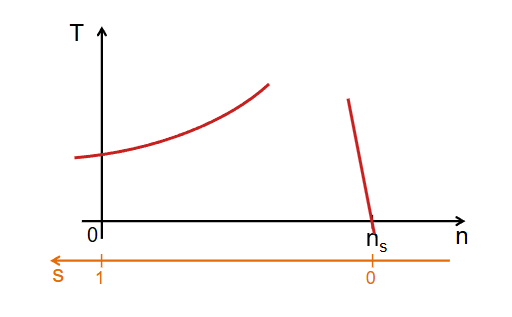
\includegraphics[width=0.5\textwidth]{assets/TNkarakteristiekzonderkippiek.png}
  \caption{T-n karakteristiek van de inductiemachine zonder het kipkoppel aangeduid}
  \label{fig:TNkarakteristiekzonderkippiek.png}
 \end{figure}

Formules voor de kipslip en het kipkoppel zijn:
\begin{align*}
    s_{kip} = \frac{R_2}{\sqrt{R_{TH}^2 + (X_{TH} + X_2)^2}} \\
    T_{kip} = \frac{3}{\omega_s} \cdot \frac{V_{TH}^2}{2[R_{TH} + \sqrt{R_{TH}^2 + (X_{TH} + X_2)^2}]}
\end{align*}
We zien dus dat de kipslip afhankelijk is van de rotorweerstand $R_2$ en niet van de
spanning!
En het geïnduceerd koppel ook maar deze is wel ook afhankelijk van de spanning
($T_{ind} \propto V_{TH}^2$) (en $V_\phi \approx V_{TH}$).
Dit is belangrijk want dit betekent dat we het koppel kunnen regelen door de spanning te
regelen, dit is eigelijk ook wel nadelig bij bvb.
spanningsdips.

\subsection{Variaties in de T-n karakteristiek}
Nu gaan we kijken naar een paar factoren die invloed kunnen hebben op de
koppel-toerentalkarakteristiek van de inductiemachine.

\subsubsection{Statorspanning}
Dus we weten nu dat het koppel afhankelijk is van de spanning in het kwadraat
($T \approx V_\phi^2$).
Bij een spanningsdip kan dit dus problematisch zijn, door dit kwadraat gaat het koppel rap
sterk dalen dan en afhankelijk van welke toepassing je de inductiemachine gebruikt kan dit
problematisch zijn.
We zullen is aan de hand van volgende grafiek bespreken wat er precies gebeurt bij zo een
spanningsdip:

\begin{figure}[H]
  \centering
  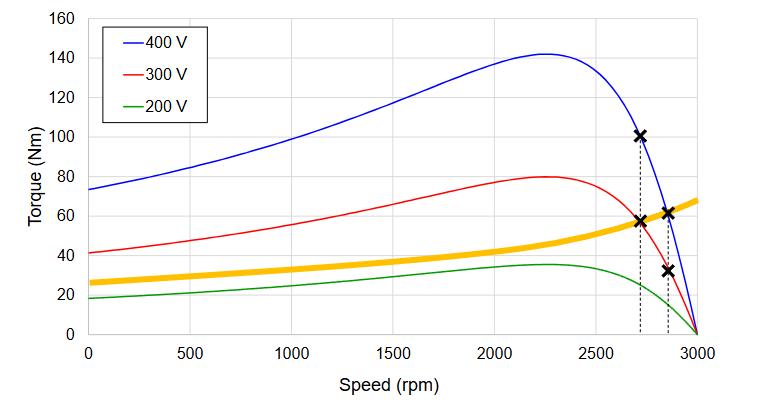
\includegraphics[width=0.6\textwidth]{assets/TNkarakteristiekverschillendespanningenenlastkarakteristiek.png}
  \caption{T-n karakteristiek bij verschillende spanningen + de lastkarakteristiek}
  \label{fig:TNkarakteristiekverschillendespanningenenlastkarakteristiek.png}
 \end{figure}

Stel we hebben 400V en een spanningsdip brengt ons naar 300V zoals in bovenstaande figuur,
dan zien we dat ons stabiel werkingspunt eerst naar beneden zakt want van zodra de
spanningsdip gebeurt is ons motor nog op dezelfde snelheid, daarna zien we echter dat onze
snelheid zal moeten vertragen tot een nieuw evenwicht voor onze last.
Hier bij die 300V is dit nog niet zo erg zien we want zodra de spanningsdip over is kunnen
we terug naar ons vorig evenwicht gaan.
Het is pas een probleem als we niet genoeg koppel meer hebben om de last te kunnen blijven
aandrijven zoals bevoorbeeld als onze spanningsdip tot die 200V daar gaat, dit is onder
die gele last karakteristiek.
Dus de spanningsdip is dan zo laag dat de motor kan uitvallen.

\subsubsection{Rotorweerstand}
We zagen dus eerder dat ons koppel ook afhankelijk is van de rotorweerstand $R_2$.
Dit kan handig zijn soms, want als we deze weerstand groter kunnen maken kunnen we een
groter startkoppel hebben en vooral dan ook een \textbf{lagere startstroom}.
Terwijl ons maximaal koppel hetzelfde blijft (wel meer slip dus meer slipverliezen).
Dit kunnen we toepassen met 'rotorweerstanden' zoals in de volgende figuren:

\begin{figure}[H]
  \centering
  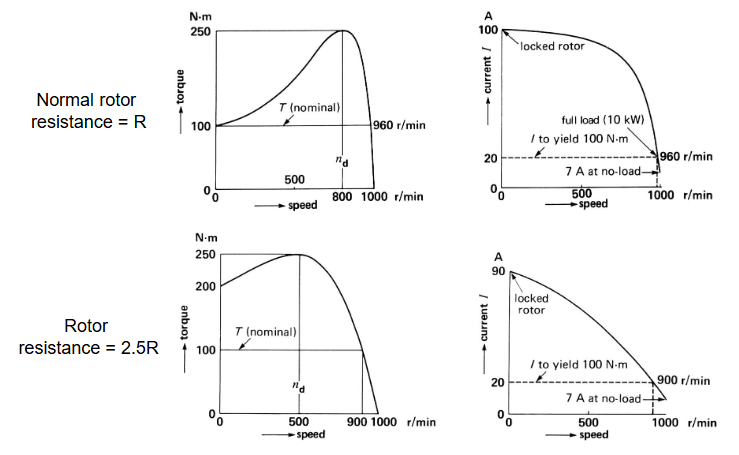
\includegraphics[width=0.7\textwidth]{assets/rotorweerstand1.png}
  \caption{Rotorweerstanden R en 2.5R}
  \label{fig:rotorweerstand1.png}
 \end{figure}

\begin{figure}[H]
  \centering
  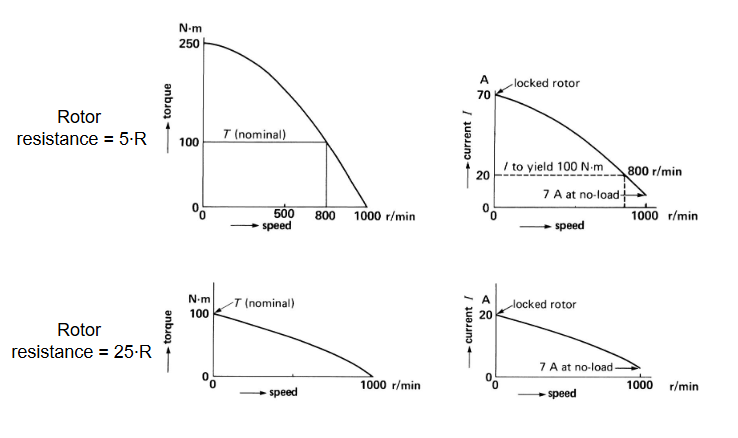
\includegraphics[width=0.7\textwidth]{assets/rotorweerstand2.png}
  \caption{Rotorweerstanden 5R en 25R}
  \label{fig:rotorweerstand2.png}
 \end{figure}

We zien dus dat bij grotere rotorweerstanden het startkoppel groter wordt en de
startstroom kleiner.
Maar wat we ook zien is dat de snelheid voor het nominaal koppel gaat dalen, soms zelfs zo
hard dat dit niet meer interessant is als je de motor op die snelheid continu wilt laten
werken.
Eigelijk willen we liefst bij opstart een grotere rotorweerstand om grotere lasten te
kunnen overwinnen maar voor ons nominaal koppel willen we een kleinere rotorweerstand.
Om dit te doen maken we gebruik van een \textbf{gewikkelde rotor} zodat we de wikkelingen
van de rotor via de sleepringen dan langs buiten kunnen aansluiten aan weerstanden (of
kortsluiten).
Ook kunnen zo die weerstanden langs buiten makkelijker gekoeld worden.

\begin{figure}[H]
  \centering
  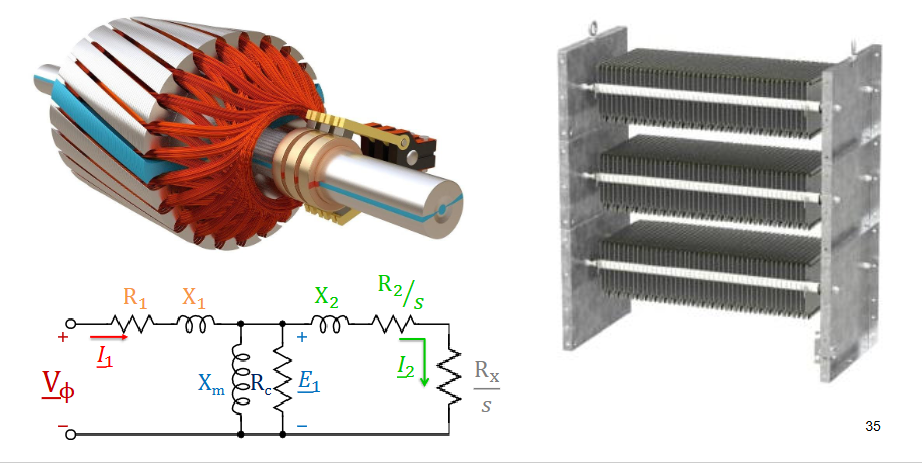
\includegraphics[width=0.6\textwidth]{assets/gewikkelderotormetweerstandenencircuitenkoelsysteem.png}
  \caption{Gewikkelde rotor met weerstanden en circuite en koelsysteem}
  \label{fig:gewikkelderotormetweerstandenencircuitenkoelsysteem.png}
 \end{figure}

Wat we ook kunnen doen is een ander soort rotor gebruiken.
De NEMA-klassen classificeren rotors (motoren eigelijk) op basis van hun kopel, je kan
hier dus ook naar kijken en kiezen.
Je kan bevoorbeeld een dubbele kooi rotor hebben.
Deze zorgen voor veel weerstand zodat je een groot startkoppel hebt en hebben eigelijk ook
een soort van adaptieve weerstand (ze zijn groter bij start), op de volgende figuur zie je
karakteristieken van een paar van die verschillende klasse motoren, sommige hebben een
\textbf{zadelpunt}:

\begin{figure}[H]
  \centering
  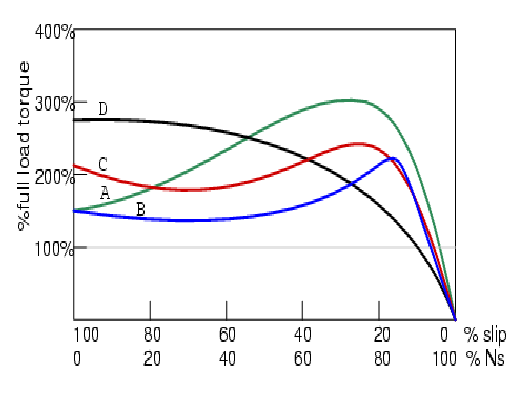
\includegraphics[width=0.5\textwidth]{assets/karakteristiekenmotorsnema.png}
  \caption{Karakteristieken van NEMA-klassen motoren}
  \label{fig:karakteristiekenmotorsnema.png}
 \end{figure}

Een \textbf{dubbele kooi rotor} heeft dus 2 kooien, een binnenste en een buitenste.
De buitenste kooi heeft een hoge weerstand en een lage inductantie, deze zorgt voor een
groot startkoppel.
De binnenste kooi heeft een lage weerstand en een hoge inductantie, deze zorgt voor een
hoog nominaal koppel.
Het nadeel van deze motoren is dat ze duurder zijn dan de standaard motoren.

\begin{figure}[H]
  \centering
  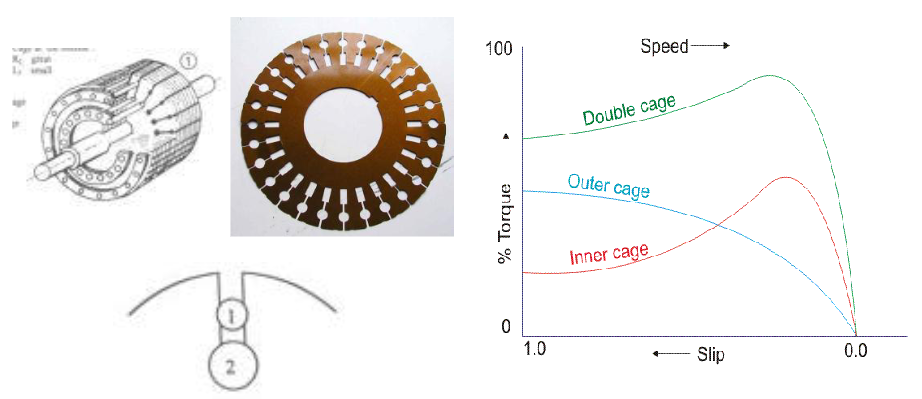
\includegraphics[width=0.8\textwidth]{assets/dubbelekooirotor.png}
  \caption{Dubbele kooi rotor}
  \label{fig:dubbelekooirotor.png}
 \end{figure}

\subsubsection{Uitgebreide T-n karakteristiek}
De formule die we eerder hadden afgeleid hadden we toen gebruikt voor onze T-n
karakteristiek, maar eigelijk werkte die formule even goed om die karakteristiek uit te
breiden zoals in de volgende figuur:

\begin{figure}[H]
  \centering
  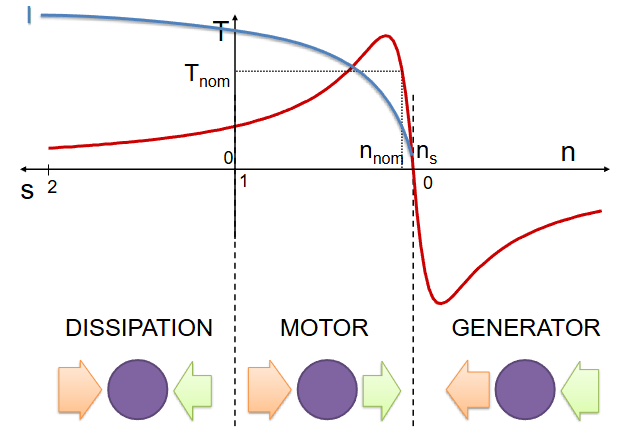
\includegraphics[width=0.5\textwidth]{assets/uitgebreideTNkarakteristiekIM.png}
  \caption{Uitgebreide T-n karakteristiek}
  \label{fig:uitgebreideTNkarakteristiekIM.png}
 \end{figure}

Deze curve komt dus ook van die formule en is even correct, we zien hier namelijk ook de
generatorwerking gedeelte van de curve, hier hebben we nog steeds een positieve snelheid
maar nu bij een negatief koppel en negatieve slip.
Wat we ook nog kunnen hebben is \textbf{dissipatie} hier sturen we eigelijk 2 vermogens de
machine in zoals je ziet bij die pijlen (de oranje pijl is het elektrisch vermogen, de
groene pijl is het mechanisch vermogen).
De slip is hier ook groter dan 1, alles wordt hier omgezet in warmte.
Op deze figuur zien we ook de curve van de strool en is het duidelijk dat we grote
startstromen hebben bij een grote slip, dit is dus ook de reden waarom we niet in dat
onstabiel gebied willen werken.

\subsubsection{4 kwadranten werking}
We kunnen deze curve eigelijk opdelen in 4 kwadranten als volgt:

\begin{figure}[H]
  \centering
  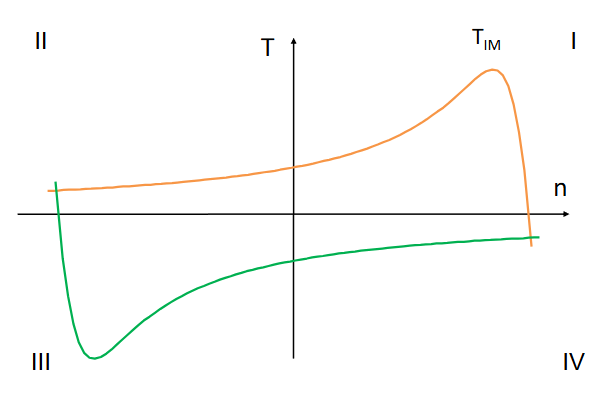
\includegraphics[width=0.6\textwidth]{assets/4kwadrantenwerking.png}
  \caption{T-n curve 4 kwadranten}
  \label{fig:4kwadrantenwerking.png}
 \end{figure}

Dit is gewoon hetzelfde als we eerder zagen maar 2 keer getekend, de oranje curve is de
nomrale T-n karakteristiek van de motor met ook de negatieve n en negatieve T nog een
beetje getoond.
De groene curve is exact hetzelfde maar $180^\circ$ gedraaid rond de oorsprong, dit
bekrijg je door 2 van de 3 fasen te wisselen (draaiveld omkeren), dit is dus het
spiegelbeeld.
De T en n-as verdelen zo het vlak in 4 kwadranten (I,II,III,IV).
De figuur toont dus eigelijk (als je beide curves samen bekijkt) dat de as van de machine
in elke combinatie van draairichting en koppelrichting terecht kan komen (de 4
kwadranten).
Om in het 3de kwadrant te komen moet je dus gewoon 2 van de 3 fases wisselen.
Daar waar die 2 curves snijden in het 4de kwadrant, dus vanaf een bepaalde snelheid, kan
je in generator werking zitten.
(Anders is de rest van dat kwadrant, en dus ook kwadrant 2, dissipatie)

\subsubsection{Ongebalanceerde voeding}
Een onbalans van het net kan ook invloed op het koppel hebben.
Eerder gingen we er altijd vanuit dat ons net in balans was (3 fases met zelfde amplitude
en verschuiving), bij onbalans op het net is dit dus niet het geval.
In vorige cursussen zagen we dat onbalans opgesplitst kan worden in 3 componenten:
de directe component, de inverse component en de homopolaire component.
Zoals we zien in volgende figuur:

\begin{figure}[H]
  \centering
  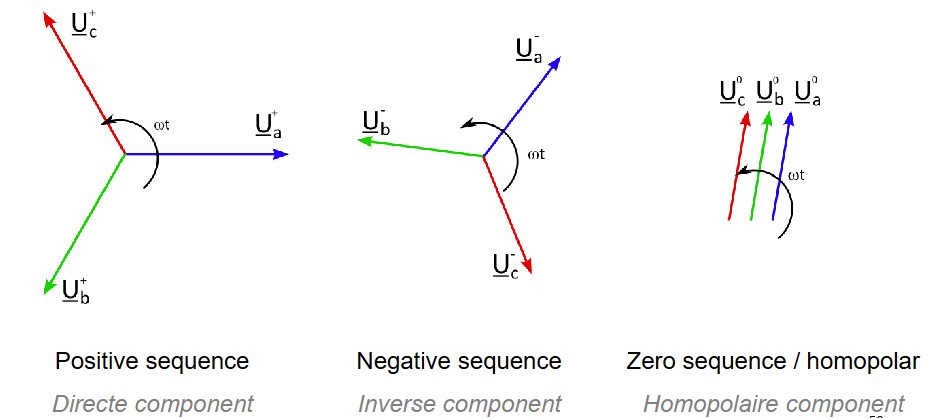
\includegraphics[width=0.7\textwidth]{assets/onbalanscomponenten.png}
  \caption{Directe, inverse en homopolaire componenten}
  \label{fig:onbalanscomponenten.png}
 \end{figure}

\begin{figure}[H]
  \centering
  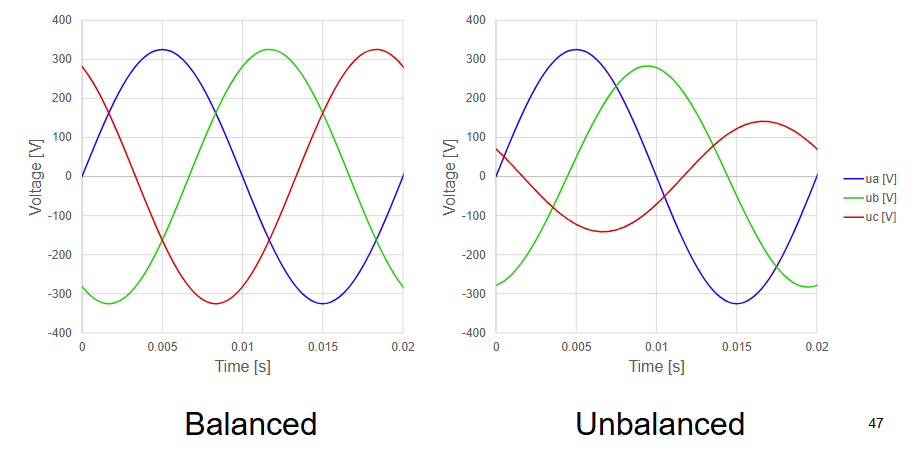
\includegraphics[width=0.6\textwidth]{assets/balancedenunbalancednet.png}
  \caption{Gebalanceerde en ongebalanceerde voeding}
  \label{fig:balancedenunbalancednet.png}
 \end{figure}

De directe component loopt zoals normaal en is ook meestal de grootste, de inverse
component loopt in tegengestelde richting en is meestal kleiner, de homopolaire component
heeft alle vectoren op één lijn liggen, hier is geen faseverschuiving tussen.
De directe maakt een draaiveld in de ene richting terwijl de indirecte die in de andere
richting maakt (de homopolaire maakt dus GEEN draaiveld), hierdoor gaan we een
ellipsvormig draaiveld krijgen als resulterende van al deze componenten.

\begin{figure}[H]
  \centering
  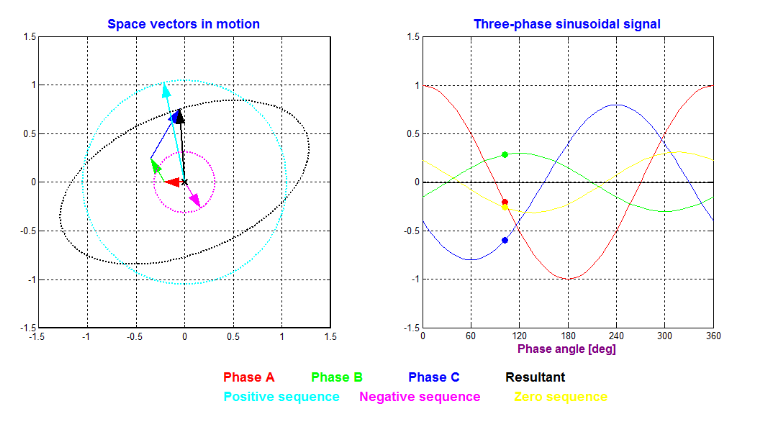
\includegraphics[width=0.6\textwidth]{assets/elliptischdraaiveld.png}
  \caption{Elliptisch draaiveld}
  \label{fig:elliptischdraaiveld.png}
 \end{figure}

Wat is nu dat effect van het elliptisch draaiveld op de T-n karakteristiek?
Bekijk deze figuur, het is eigelijk de 4 kwadrant operatie:

\begin{figure}[H]
  \centering
  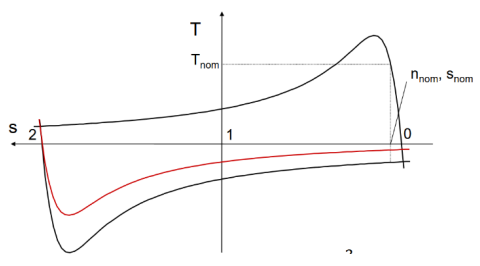
\includegraphics[width=0.6\textwidth]{assets/4kwadrantoperatiedirectenondirectecomponent.png}
  \caption{4 kwadrant operatie met directe en inverse component}
  \label{fig:4kwadrantoperatiedirectenondirectecomponent.png}
 \end{figure}

Die bovenste T-n karakteristiek is de normale karakteristiek, deze wordt gemaakt door de
directe component.
De onderste gespiegelde dan door de inverse component.
Doordat de 2 koppels een andere amplitude kunnen hebben moeten deze dus ook geschaald
worden als we het totale koppel willen bepalen, dit wordt dan gedaan met de volgende
formule:
\begin{align*}
 T(s) = T_{+}(s) \cdot |{\frac{V_{+}}{V_{\phi}}}|^2 + T_{-}(s) \cdot |{\frac{V_{-}}{V_{\phi}}}|^2
\end{align*}
Want het koppel heeft een kwadratisch verband met de spanning.
We willen zo weinig mogelijk van de inverse component want zoals we ziet zit die in
dissipatie, dus dit brengt alleen extra hitte met zich mee.
En dus ook zien we dat dit eigelijk een negatieve koppel is en zich dus aftrekt van het
koppel van de directe component.
Een onbalans kan dus het koppel licht doen verlagen maar zorgt wel voor veel extra
opwarming.

\begin{figure}[H]
  \centering
  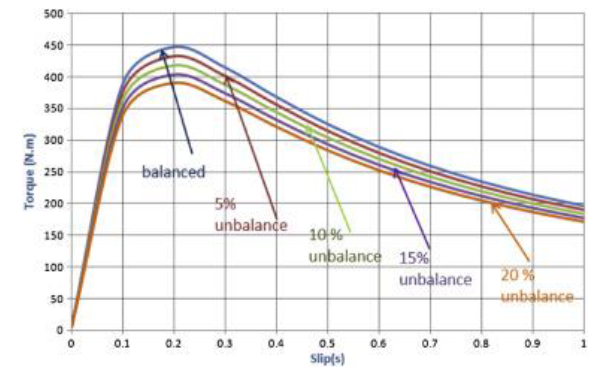
\includegraphics[width=0.6\textwidth]{assets/weergavekoppelverliesdooronbalans.png}
  \caption{Weergave koppelverlies door onbalans}
  \label{fig:weergavekoppelverliesdooronbalans.png}
 \end{figure}

Hierboven zie je dus hoeveel koppel je verliest met hoeveel percentage onbalans, niet
super veel dus, niet problematisch.
In de figuur hieronder zie je de temperatuurinvloed door onbalans, dit is duidelijk wel
problematisch want dit doet de levensduur zakken.
Je ziet dat een onbalans van slechts 3.5\% al voor een temperatuurverschil van 25\% kan
zorgen.

\begin{figure}[H]
  \centering
  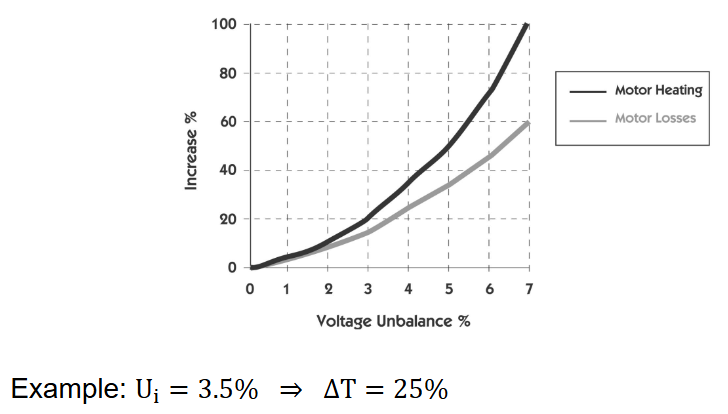
\includegraphics[width=0.5\textwidth]{assets/tempeffectonbalans.png}
  \caption{Temperatuur-effect van onbalans}
  \label{fig:tempeffectonbalans.png}
 \end{figure}

Wat is nu het effect van die homopolaire component?
De homopolaire component is eigelijk 3 keer hetzelfde, het is dus eigelijk een 1-fasige
wisselspanning en dit kan ook een koppel genereren, alleen kan het niet zelf starten:

\begin{figure}[H]
  \centering
  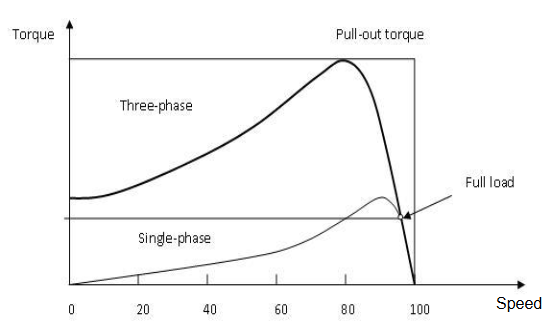
\includegraphics[width=0.6\textwidth]{assets/Tn3fasigen1fasig.png}
  \caption{Weergave koppel door homopolaire component}
  \label{fig:Tn3fasigen1fasig.png}
 \end{figure}

Maar eigelijk gedraagt zich dit als 3 enkelfasige motors waardoor we 3 keer zoveel polen
hebben en dus een veel vroegere synchrone snelheid dan de directe en inverse component.
Dit maakt dat we al rap in generatorwerking gaan zitten, wat een nefatieve invloed heeft,
zoals we zien in volgende figuur:

\begin{figure}[H]
  \centering
  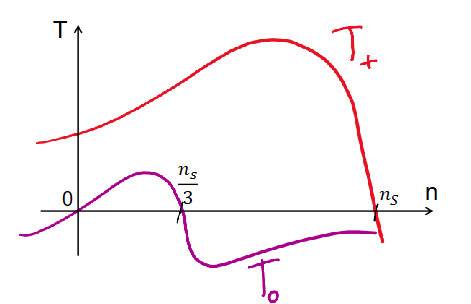
\includegraphics[width=0.5\textwidth]{assets/TNdirecteenhomopolairecomponent.png}
  \caption{T-n karakteristiek van de directe en homopolaire component}
  \label{fig:TNdirecteenhomopolairecomponent.png}
 \end{figure}

De echte formule voor $T(s)$ met de homopolaire component wordt dan:
\begin{align*}
 \boxed{T(s) = T_{+}(s) \cdot |{\frac{V_{+}}{V_{\phi}}}|^2 + T_{-}(s) \cdot |{\frac{V_{-}}{V_{\phi}}}|^2 + T_{0}(s) \cdot |{\frac{V_{0}}{V_l / 3}}|^2}
\end{align*}
Echter is die homopolaire component geen probleem want je kan die makkelijk wegwerken/niet
laten mee tellen door je sterpunt zwevend te laten (geen Neutraal (N) aan te sluiten) in
je sterschakeling, of door sowieso een driehoekschakeling te gebruiken (die heeft toch
geen sterpunt).
Zonder retourpad kan er namelijk geen homopolaire stroom vloeien.

\section{Inductiemachines in gebruik}
Voor het starten van de inductiemachine is een startkoppel ($T_{start}$) en een
startstroom ($I_{start}$) nodig.
In sommige gevallen willen we een lage startkoppel, in sommige een hoge.
Hoe gaan we deze dan beperken?
We kunnen dit doen door de spanning bij opstart te verlagen, maar we willen dit maar
tijdelijk, dit doet ook de startstroom verlagen, wat goed is want deze willen we in alle
gevallen laag.
We gaan dus nu eens kijken naar verschillende manieren om deze motoren te starten.
Daarna gaan we eens kijken naar hoe we de motor remmen en tot slot naar de
generatorwerking van de inductiemachine.
Manieren om op te starten die we gaan bespreken zijn:

\begin{itemize}
 \item Directe aanloop
 \item Stator serie weerstanden
 \item Autotransformer (Spaartransformator)
 \item Softstarter
 \item Ster-driehoek starten
 \item Externe rotorweerstanden
\end{itemize}

\subsection{Directe aanloop (Direct on line, DOL)}
Dit is gewoon van het net starten met een start/stop knop via een zekering.
Dit is de opstartcurve die we eerder zagen, het heeft dus een hoge startstroom maar is
heel simpel om op te starten.
Vooral in situaties waar we niet te veel moeten opstarten of dingen die niet echt een
snelheidsregeling nodig hebben.

\begin{figure}[H]
  \centering
  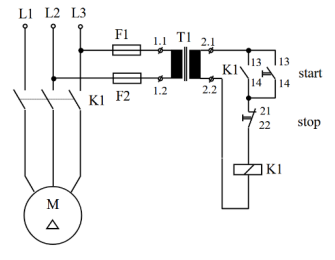
\includegraphics[width=0.5\textwidth]{assets/directeaanloop.png}
  \caption{Directe aanloop van de inductiemachine}
  \label{fig:directeaanloop.png}
 \end{figure}

\subsection{Stator serie weerstanden}
Hier gaan we regelbare weerstanden in serie zetten met de stator, bij opstarten maken we
deze weerstanden maximaal zodat er een grotere spanningsval is over de weerstand ipv de
motor, dit daalt het startkoppel en de startstroom dus.
De weerstanden worden steeds lager gemaakt tot we op nominale spanning zijn.
De weerstanden worden wel snel heel warm, deze moeten dus eigelijk gekoeld worden.

\begin{figure}[H]
  \centering
  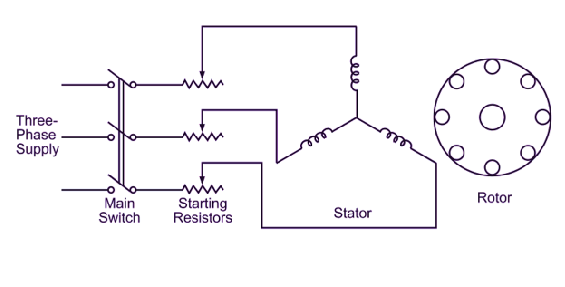
\includegraphics[width=0.6\textwidth]{assets/statorweerstandenserie.png}
  \caption{Stator serie weerstanden}
  \label{fig:statorweerstandenserie.png}
 \end{figure}

\subsection{Autotransformer (Spaartransformator)}
Een andere oplossing is opstarten met een spaartransformatie in serie met de motor, dit is
eigelijk gelijkaardig aan die stator serie weerstanden, dit gebruikt echter spoelen om
spanning te dempen, het verlagen van de opstartstroom en opstartkoppel is eigenlijk meer
'energetisch', je kan veel meer spanningsval hiermee creëren met veel minder vermogen
verlies (want dit werkt met reactief vermogen).
Maar het grote nadeel is wel dat het duur is.

\begin{figure}[H]
  \centering
  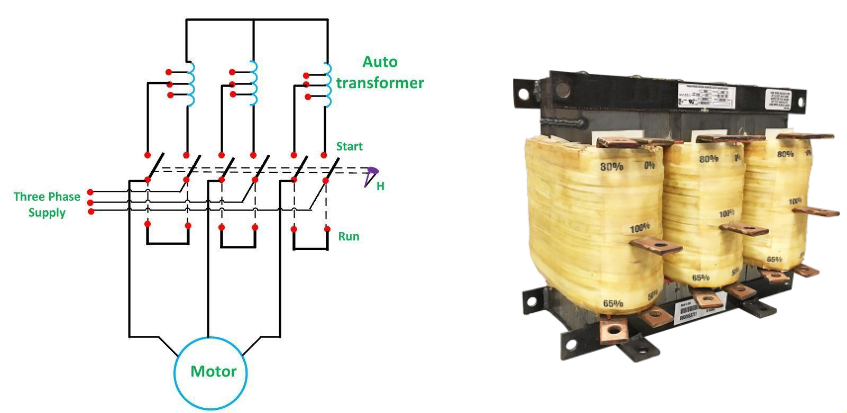
\includegraphics[width=0.6\textwidth]{assets/autotransforspaar.png}
  \caption{Autotransformer (Spaartransformator)}
  \label{fig:autotransforspaar.png}
 \end{figure}

\subsection{Softstarter}
Een softstarter is vermogenelektronica, het is meer geavanceerder en dus ook duurder.
Het gebruikt thyristors (soort van diodes) in antiparallele posities (TRIACS), deze
geleiden van zodra een signaal wordt gegeven op de gate.
Hiermee kunnen we dus eigelijk geleidelijk aan de spanning verhogen door steeds meer van
de sinus te laten doorlaten (steeds meer energie in de golf).
Dit noemt eigelijk de 'ontsteekhoek' die we steeds kleiner maken.
Dit kunnen we zien in de volgende figuur:

\begin{figure}[H]
  \centering
  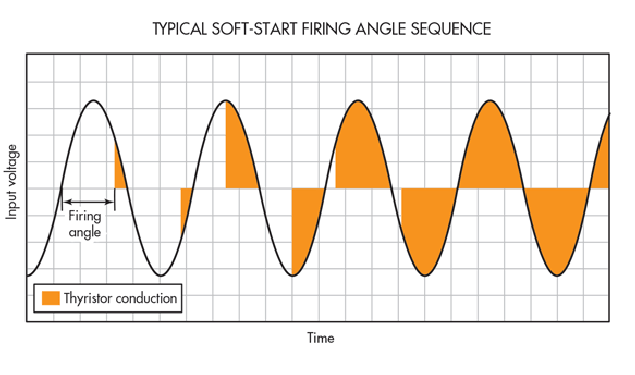
\includegraphics[width=0.6\textwidth]{assets/thyrsitorsinus.png}
  \caption{Softstarter met thyristors die geleidelijk de spanning verhogen}
  \label{fig:thyrsitorsinus.png}
 \end{figure}

\begin{figure}[H]
  \centering
  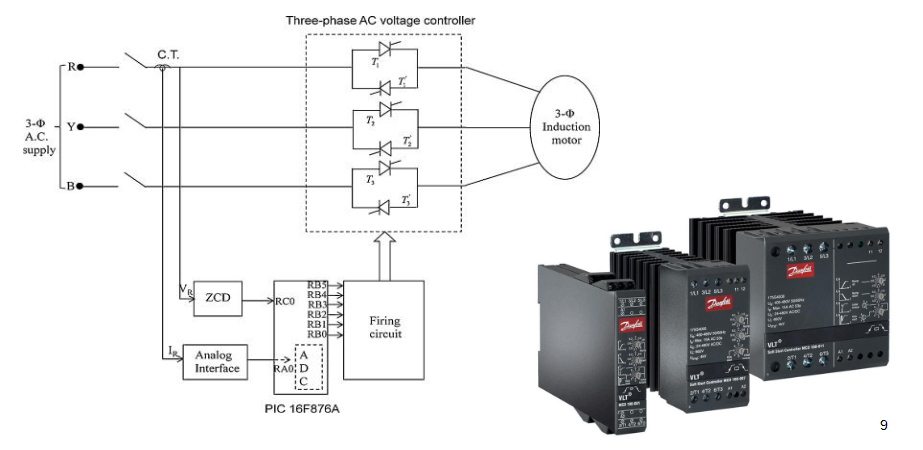
\includegraphics[width=0.6\textwidth]{assets/softstarterschakeling.png}
  \caption{Softstarter schakeling}
  \label{fig:softstarterschakeling.png}
 \end{figure}

Echter zorgt dit wel voor veel harmonischen (extra opwarming), maar dit is nog steeds
beter dan hoge startstromen.
Maar omdat het nog steeds warm is worden er koelvinnen op de softstarter geplaatst.

\subsection{Ster-driehoek starten}
De goedkoopste methode is ster-driehoek starten, hiervoor gebruik je gewoon een schakelaar
en 2 contactoren (ookal zijn contactoren nog wel duur).
We starten hierbij gewoon in ster, want in ster is de fasespanning lager
($V_f = \frac{V_L}{\sqrt{3}}$) en dus het startkoppel 3 keer lager (want
$T \propto V_f^2 \propto \frac{V_L^2}{3}$).
Het zelfde geld met de stroom want als je van ster naar driehoek gaat dan stijgt de
spanning met $\sqrt{3}$ en de stroom ook met $\sqrt{3}$ dus samen stijgt de stroom met een
factor van 3.
(Dit is belangrijk om door te hebben!).

\begin{figure}[H]
  \centering
  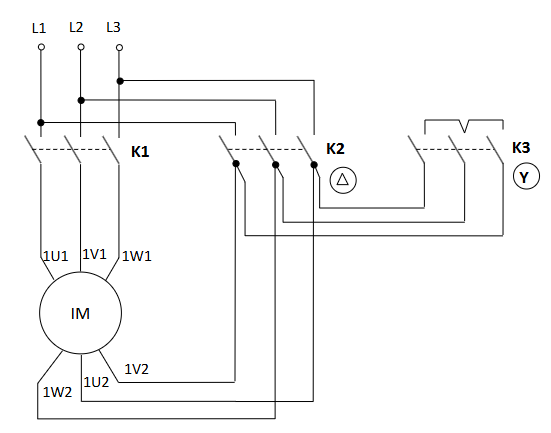
\includegraphics[width=0.5\textwidth]{assets/sterdriehoekstartenschakeling.png}
  \caption{Schakeling voor ster-driehoek starten}
  \label{fig:sterdriehoekstartenschakeling.png}
 \end{figure} 

Uiteindelijk willen we dus in driehoek werken, want zo zitten we op ons volledig vermogen.
Op het moment van starten sluiten we K1 en K3, na een verloop van tijd gaan we EERST K3
openen (ster uitzetten) en dan K2 sluiten zodat we in driehoek zitten.
We openen eerst K3 omdat we anders een kortsluiting op het net veroorzaken als we K2
sluiten als K3 nog gesloten is.
Dit kan voorkomen worden dat dit gebeurd als we gewoon normally closed en normally open
contactoren hiervoor gebruikt worden.
Een nadeel is wel door dit te schakelen dat we eigelijk een transiënte krijgen, dit zien
we in volgende karakteristiek voor ster en driehoek schakelen:

\begin{figure}[H]
  \centering
  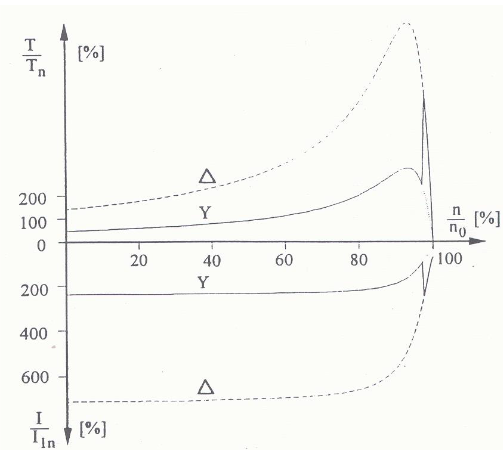
\includegraphics[width=0.5\textwidth]{assets/karakteristieksterdriehoekschakele.png}
  \caption{Karakteristiek van ster-driehoek schakelen}
  \label{fig:karakteristieksterdriehoekschakele.png}
 \end{figure}

Hier zien we deze transiente beter in een I-t karakteristiek:

\begin{figure}[H]
  \centering
  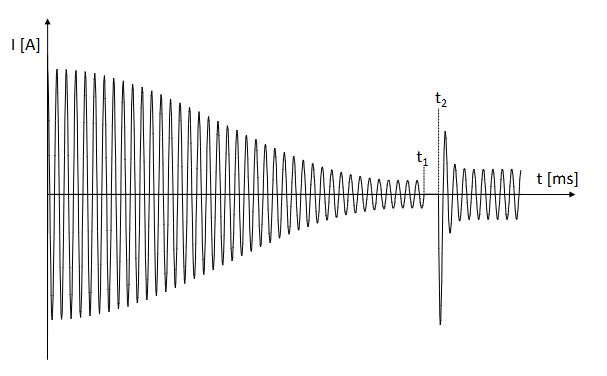
\includegraphics[width=0.6\textwidth]{assets/trabsiente.png}
  \caption{Transiënte karakteristiek bij ster-driehoek schakelen}
  \label{fig:trabsiente.png}
 \end{figure}

Dit kan verminderd worden door te werken met een tijdsvertraging.

\subsubsection{Vergelijken met DOL en Softstarter}
We gaan dan nu is de stroom en koppelkarakteristieken van de DOL, softstarter en
ster-driehoek vergelijken.
Dit zien we in de volgende figuur:

\begin{figure}[H]
  \centering
  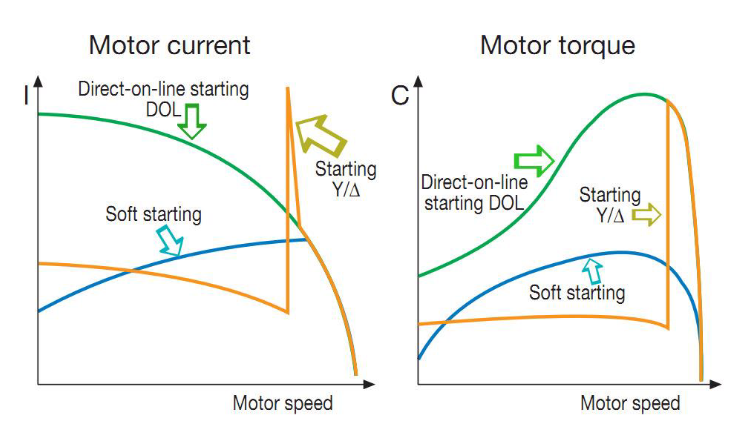
\includegraphics[width=0.6\textwidth]{assets/stroomkoppeldolsoftstartersterdriehoek.png}
  \caption{Stroom en koppelkarakteristieken van DOL, softstarter en ster-driehoek}
  \label{fig:stroomkoppeldolsoftstartersterdriehoek.png}
 \end{figure}

Nu zien we ook waarom softstarter 'soft' starter heet, je ziet dat de start voor de stroom
en koppel mooi geleidelijk is, het heeft een vlak profiel.
De ster-driehoek is een beetje vergelijkbaar maar je ziet hier wel duidelijk die
transiënte waardoor het koppel eigelijk een lichte schok krijgt, wat je dus niet hebt bij
de softstarter.
(De proff meld wel nog dat de transiëntes hier een beetje overdreven getekend zijn)

\subsection{Externe rotorweerstanden}
Wat als we een hoge startkoppel willen maar geen hoge startstroom?
Dan kunnen we gebruik maken van externe rotorweerstanden.
Hiervoor is dus wel een gewonden rotor nodig (dit zagen we eerder, want hieraan kan je via
sleepringen die weerstanden hangen).
Bekijk nu eens volgende figuur:

\begin{figure}[H]
  \centering
  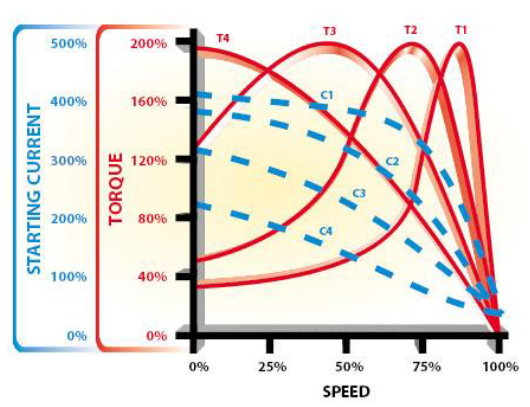
\includegraphics[width=0.6\textwidth]{assets/startstroomenstartkoppelbijverschillenderotorweerstanden.png}
  \caption{Startstroom en startkoppel bij verschillende rotorweerstanden}
  \label{fig:startstroomenstartkoppelbijverschillenderotorweerstanden.png}
 \end{figure}

Wat we gaan doen is dus beginnen bij T4, dit heeft dus een lage startstroom en hoog
startkoppel, naarmate de snelheid toeneemt zullen het koppel en de stroom dus dalen.
Wat we gaan doen is dan schakelen naar T3 (de volgende rotorweerstand), dit zorgt ervoor
dat ons koppel niet begint te dalen maar ongeveer hetzelfde blijf, zelfde voor de stroom.
Zo gaan we dan over naar T2 en dan naar T1.
Dit zorgt dat we een langere tijd een hoog koppel hebben met een lage stroom.
Dit is mogelijk volgens de formule voor $T_{ind}$ die we ook eerder zagen.
Nadeel is dus dat je een gewikkelde rotor nodig hebt wat duur is, dit is niet toepasbaar
bij een kooirotor.
Een schema hiervan ziet er zo uit:

\begin{figure}[H]
  \centering
  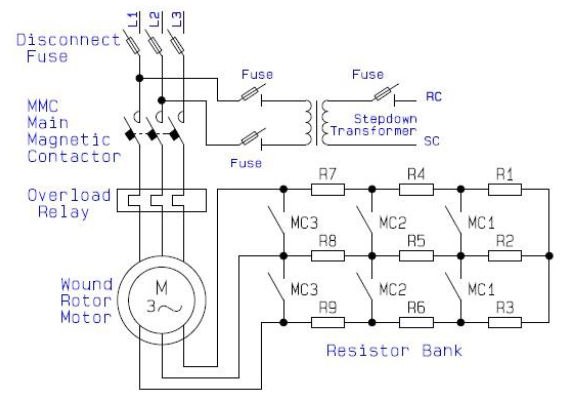
\includegraphics[width=0.5\textwidth]{assets/externerotorweerstandenschema.png}
  \caption{Schema van externe rotorweerstanden}
  \label{fig:externerotorweerstandenschema.png}
 \end{figure}

\subsection{Remmen van de inductiemachine}
Nu gaan we kijken naar het remmen van de inductiemachine.
We hebben 5 soorten remmen voor de inductiemachine zonder gebruik te maken van externe
remmen (dat niet gewoon uitbollen zijn).
Deze zijn:

\begin{itemize}
    \item Plugging (tegenstroom remmen)
    \item DC-remmen
    \item Zero sequence braking (Homopolair remmen)
    \item Oversynchroon remmen
    \item Regeneratief remmen
\end{itemize}

\subsubsection{Plugging (tegenstroom remmen)}
Wat we hier gaan doen is eigelijk op ons stabiel werkingspunt de hoofdschakelaar
uitschakelen en dan een andere schakeling aanzetten waarbij 2 fases omgedraaid zijn ten
opzichte van de hoofdschakkelaar, zodat we eigelijk in het 4de kwadrant terecht komen in
dissipatie, dit remt sterk af.
We moeten hier wel zien dat we op tijd die schakelaar dan ook uitzetten want anders gaan
we gewoon in de andere richting versnellen.
Dit wordt vooral toegepast als we snel gestopt kunnen raken en niet te veel moeten stoppen
want dit warmt veel op door die dissipatie.

\begin{figure}[H]
  \centering
  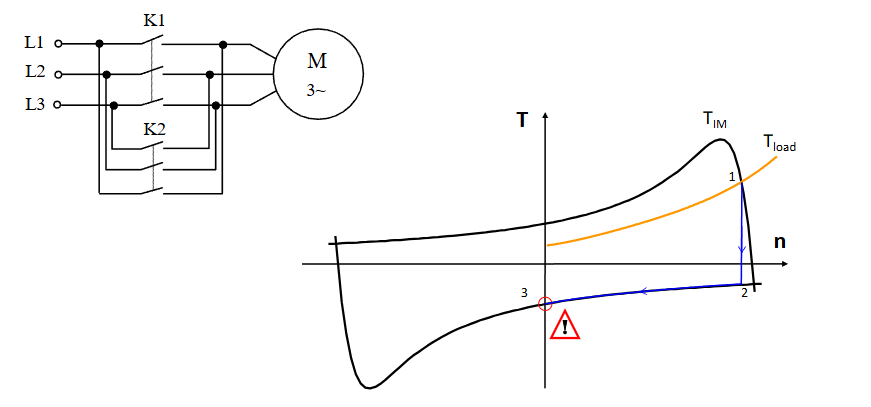
\includegraphics[width=0.6\textwidth]{assets/tegenstroomremmen.png}
  \caption{Tegenstroomremmen}
  \label{fig:tegenstroomremmen.png}
 \end{figure}

Dit is de goedkoopste remmethode, het heeft een 2de contactor nodig.
Om te checken dat je op tijd de andere contactor sluit zodat je niet versnelt gebruiken we
een 'ruwe' snelheidsdetectie, deze heeft een accuraatheid dat 50 tr/min kan schelen.

\subsubsection{DC-remmen}
Deze methode wordt minder gebruikt omdat een gelijkstroomrichter nodig is dat wat duurder
is, maar bij niet te grote vermogens valt dit goed mee.
Wat we hier gaan doen is met een gelijkstroombron (DC) een gelijkstroom aanleggen op 2
windingen zodat we in de stator een constant magnetisch veld krijgen (dus geen draaiveld),
dit gaat in de rotor een spanning induceren dat een stroom veroorzaakt en dus een koppel
genereert dat tegengesteld is aan de draairichting van de rotor.
Dit remt dus af.
Wat we ook zien is dat dit koppel toeneemt naarmate de rotor afremt en dat deze gelijk is
aan 0 als de snelheid 0 is, dit lost dus het probleem van de vorige methode op.

\begin{figure}[H]
  \centering
  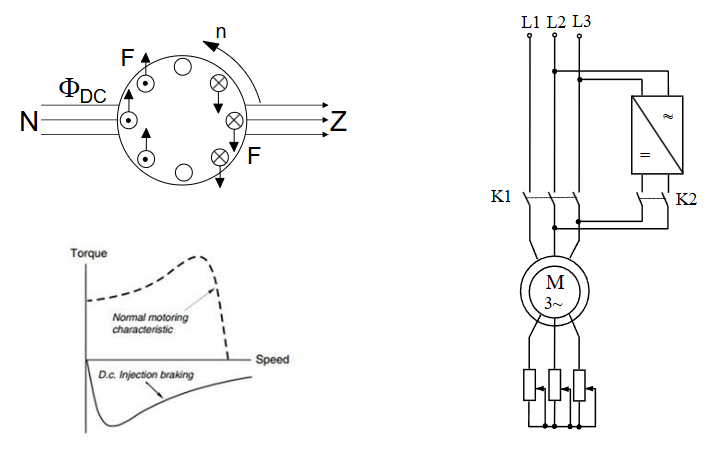
\includegraphics[width=0.5\textwidth]{assets/DCremmen.png}
  \caption{DC-remmen}
  \label{fig:DCremmen.png}
 \end{figure}

\subsubsection{Zero sequence braking (Homopolair remmen)}
Dit is maar kort besproken in de les, maar wat we hier doen is de motor loskoppelen van
het net en de 3 statorwikkelingen aansluiten zodat ze allemaal exact dezelfde stroom met
dezelfde fase (homopolair) krijgen want tegenover de draaiened rotor geeft dit netto een
afremmend koppel die we eerder zagen.

\subsubsection{Oversynchroon remmen}
Dit wordt eigelijk minder als remmen beschouwt, dit is eerder om te voorkomen dat iets
beweegt of te snel gaat.
Vooral gebruikt in liften/kranen.
Bij lasten laten zakken gaan we eigelijk gewoon in generatorwerking gaan en dus een
negatief koppel krijgen wat doet afremmen.
Potentiele energie wordt dus terug omgezet in elektrische energie, dit maakt het een soort
van generatief remmen.

\begin{figure}[H]
  \centering
  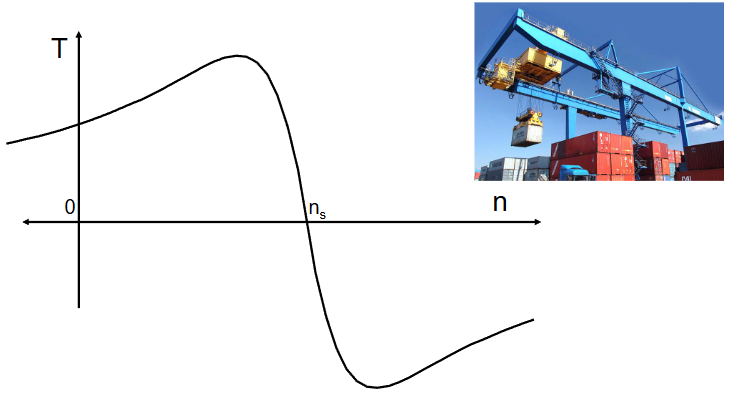
\includegraphics[width=0.5\textwidth]{assets/oversynchroonremmen.png}
  \caption{Oversynchroon remmen}
  \label{fig:oversynchroonremmen.png}
 \end{figure}

\subsubsection{Regeneratief remmen}
Hierbij gaan we echt remmen door gebruik te maken van de generatorwerking van de
inductiemachine.
Hiervoor moeten we de synchrone snelheid verlagen zodat de curve naar links opschuift
zoals je ziet in de figuur.
De rotor beweegt zo sneller als het magnetisch veld wat dus generator werking veroorzaakt.
Dit gaan we doen door de flux constant te houden en de frequentie aanpassen met een
frequentieregelaar.
Maar omdat frequentie aanpassen het veld aanpast (dat we constant willen houden) gaan we
samen de spanning met de frequentie doen dalen want $E \approx V_\phi$ en dit doen we dan
stap per stap.

\begin{figure}[H]
  \centering
  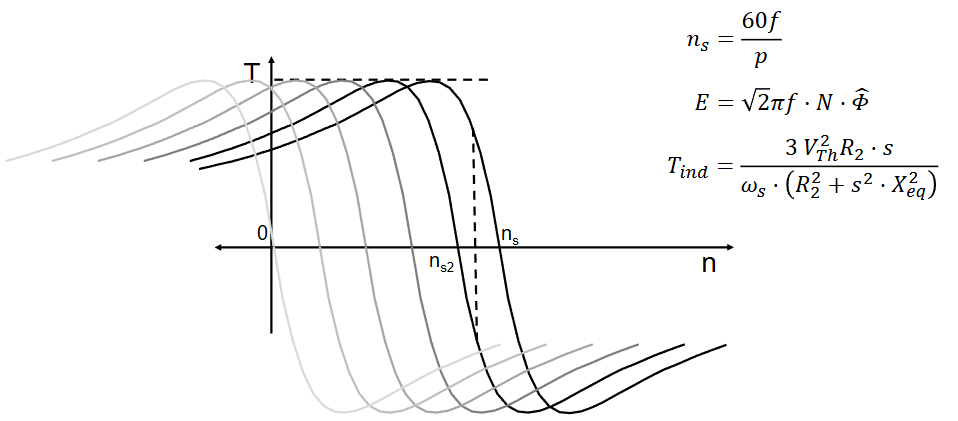
\includegraphics[width=0.7\textwidth]{assets/regeneratiefremmen.png}
  \caption{Regeneratief remmen}
  \label{fig:regeneratiefremmen.png}
 \end{figure}

\subsection{Generatorwerking van de inductiemachine}
Nu gaan we eens kijken naar de generatorwerking van de inductiemachine.
Het is het gedeelte $\frac{R_2}{s}$ dat ervoor zorgt dat als we negatieve slip hebben dat
er energie geleverd wordt door magnetisch veld naar de stator.
We gaan eens kijken naar een wind turbine:

\begin{figure}[H]
  \centering
  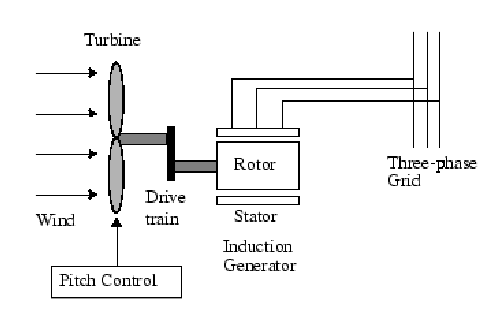
\includegraphics[width=0.5\textwidth]{assets/windturbinevoorbeeld.png}
  \caption{Windturbine voorbeeld}
  \label{fig:windturbinevoorbeeld.png}
 \end{figure}

Dit is een grote generator, wat het doet is eigelijk actief vermogen tot het net brengen.
De motor kan alleen actieve energie leveren terwijl de rotor ook reactief vermogen nodig
heeft in de wikkelingen voor het veld te maken, het moet dit dus van het net trekken,
daarvoor worden condensator banken gebruikt, deze verminderen het reactief vermogen dat we
van het net moeten nemen.
De reden dat dit met een asynchrone en niet een synchrone machine is, is omdat dit niet op
een constante snelheid werkt.
Ook is er nog een overbrenging om de rotatie naar een ideale snelheid voor de motor te
brengen.

\subsubsection{Singly Fed}
Dit is het normale geval, enkel de stator is hier elektrisch aan het net gesloten.
De rotor krijgt stroom via inductie.
Dit is gewoon de standaard generator werking die we eerder zagen.

\begin{figure}[H]
  \centering
  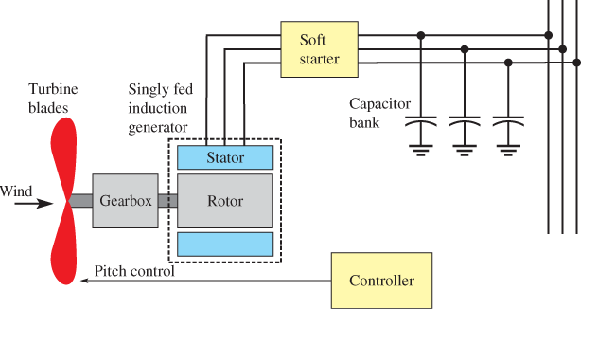
\includegraphics[width=0.6\textwidth]{assets/singlyfed.png}
  \caption{Singly Fed}
  \label{fig:singlyfed.png}
 \end{figure}

\subsubsection{Doubly Fed}
Dit is al wat anders.
Hier beide wikkelingen elektrisch aangesloten.
Zowel de stator als rotor aan het net dus.
We gaan zoveel mogelijk actief vermogen naar het net sturen.
Voor de rotor wordt hier vermogenelektronica en rotor weerstanden gebruikt zodat je een
optimaal koppel behoudt en zoveel mogelijk naar het net kan sturen.
Dit is veel efficiënter.

\begin{figure}[H]
  \centering
  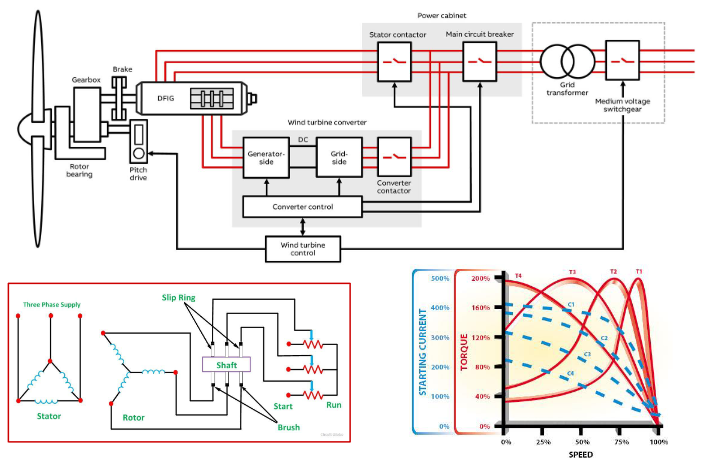
\includegraphics[width=0.6\textwidth]{assets/doublyfed.png}
  \caption{Doubly Fed}
  \label{fig:doublyfed.png}
 \end{figure}

\subsection{Oefeningen}

\begin{oefenblok}[Oefening 6-26 Slides]
    \textbf{Opgave:}
    \newline
    A 460V 50hp (=37kW) six-pole $\Delta$-connected 60Hz threephase induction motor has a
    full-load slip of 4\%, an efficiency of 91\% and a power factor of 0.87 lagging.
    At start-up the motor develops 1.75 times the full-load torque but draws 7 times the
    rated current at the rated voltage.
    This motor is to be started at reduced voltage using a softstarter.
\begin{itemize}
 \item a) What should be the output voltage of the softstarter to reduce the starting
 torque until it equals the rated torque of the motor?
 \item b) What will the motor starting current be at this voltage?
 \item c) And what is the current drawn from the supply?
\end{itemize}
   \textbf{Oplossing:}
   \newline
   \dots ({\color{red}Nog niet aan begonnen})
\end{oefenblok}

\begin{oefenblok}[Excercise Induction motor Slides]
    \textbf{Opgave:}
    \begin{figure}[H]
      \centering
      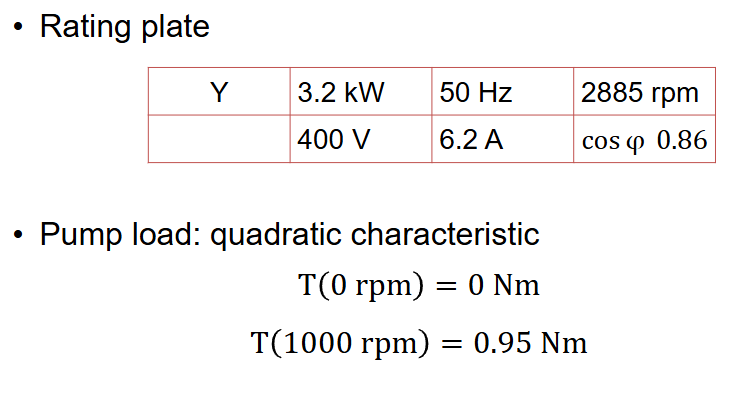
\includegraphics[width=0.6\textwidth]{assets/opgaveIMoefening.png}
      \caption{Opgave Inductie Motor}
      \label{fig:opgaveIMoefening.png}
     \end{figure}
    \begin{itemize}
     \item a) Nominal operation point
     $\rightarrow n_s, n_{nom}, s_{nom}, P_{el}, P_{mech}, \eta, T_{nom}$
     \item b) Load $\rightarrow$ operation point
     \item c) Voltage dip $\Delta U_l = 80 V \rightarrow$ torque?
    \end{itemize}
    \textbf{Oplossing:}
    \newline
    \dots ({\color{red}Nog niet aan begonnen})
\end{oefenblok}

\begin{oefenblok}[Oefening 1 - Slip (Toledo)]
    \textbf{Opgave:}
    \newline
    Slip and speed are related.
    Complete the drawing by naming the slip axis (pink) and adding some interesting
    values.
    \begin{figure}[H]
      \centering
      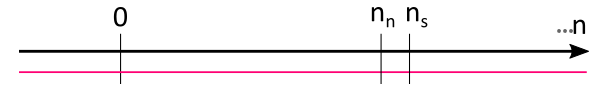
\includegraphics[width=0.6\textwidth]{assets/opgaveSlip.png}
      \caption{Opgave Slip}
      \label{fig:opgaveSlip.png}
     \end{figure}
    \textbf{Oplossing:}
    \newline
    \dots ({\color{red}Nog niet aan begonnen})
\end{oefenblok}

\begin{oefenblok}[Oefening 2 - Rating plate (Toledo)]
    \textbf{Opgave:}
    \newline
    Questions:
    \begin{itemize}
     \item 1.
     number of pole sets, synchronous speed, nominal slip, efficiency, nominal torque
     \item 2. if the torque is only $T_{nom}/2$, determine the delivered power
     \item 3. at which speed will the machine rotate if it is driven at $T=25\,Nm$?
    \end{itemize}
    Numerical answers:
    \begin{itemize}
     \item 1. 2, 1500rpm, 4\%, 81\%, 37Nm
     \item 2. 2.8kW
     \item 3. 1545rpm
    \end{itemize}
    \textbf{Oplossing:}
    \newline
    \dots ({\color{red}Nog niet aan begonnen})
\end{oefenblok}

\begin{oefenblok}[Oefening 3 - Equivalent circuit (Toledo)]
    \textbf{Opgave:}
    \newline
    Determine the equivalent circuit of an induction machine, supplied by the grid
    $3\times400V@50Hz$, with following rating plate and measurements:
    \begin{itemize}
     \item Rating plate: 400V; 50Hz; 533A; $\cos\varphi$ 0.89; 315kW; 2980rpm
     \item No load: $I_0 = 124.7\,A$; $P_0 = 5.73\,kW$;
     \item Locked rotor: $U_{lr} = 66.1\,V$; $P_{lr} = 16.3\,kW$;
     \item Full load: $P_{in} = 327.5\,kW$; $P_{out} = 315\,kW$;
     \item Resistance between lines = $4.4\,m\Omega$
    \end{itemize}
    Numerical answers:
    $R_1=2.2\,m\Omega$, $X_1=61\,m\Omega$, $X_2=61\,m\Omega$, $R_2=17\,m\Omega$,
    $R_c=28\,\Omega$, $X_m=1.8\,\Omega$
    \newline
    \textbf{Oplossing:}
    \newline
    \dots ({\color{red}Nog niet aan begonnen})
\end{oefenblok}

\begin{oefenblok}[Oefening 5 - Pump load (Toledo)]
    \textbf{Opgave:}
    \newline
    Given:
    \begin{itemize}
     \item Rating plate: 3.2kW, 50Hz, 2885rpm, 400V (Y), 6.2A, $\cos\varphi$ 0.86
     \item neglect stator losses, iron losses
     \item $I_0=2.8\,A$, $L_{leakage}=4.5\,mH$
     \item load: pump (quadratic characteristic, $T_{pump}=0.95\,Nm$ at 1000rpm)
    \end{itemize}
    Questions:
    \begin{itemize}
     \item 1. Determine: $n_s, n_{nom}, s_{nom}, P_{el}, P_{mech}, \eta_{nom}$
     \item 2.
     the (simplified) equivalent circuit:
     elements, voltages and currents.
     Draw the phasor diagram too
     \item 3. Determine the operating point when driving the pump (torque and speed)
     \item 4. For a voltage dip of 80V, determine the motor torque.
    \end{itemize}
    \textbf{Oplossing:}
    \newline
    \dots ({\color{red}Nog niet aan begonnen})
\end{oefenblok}

% ==================================================================

% ==================================================================

\newpage
